% Options for packages loaded elsewhere
% Options for packages loaded elsewhere
\PassOptionsToPackage{unicode}{hyperref}
\PassOptionsToPackage{hyphens}{url}
\PassOptionsToPackage{dvipsnames,svgnames,x11names}{xcolor}
%
\documentclass[
  english,
  letterpaper,
  numbers=noendperiod,
  DIV=13]{scrreprt}
\usepackage{xcolor}
\usepackage{amsmath,amssymb}
\setcounter{secnumdepth}{-\maxdimen} % remove section numbering
\usepackage{iftex}
\ifPDFTeX
  \usepackage[T1]{fontenc}
  \usepackage[utf8]{inputenc}
  \usepackage{textcomp} % provide euro and other symbols
\else % if luatex or xetex
  \usepackage{unicode-math} % this also loads fontspec
  \defaultfontfeatures{Scale=MatchLowercase}
  \defaultfontfeatures[\rmfamily]{Ligatures=TeX,Scale=1}
\fi
\usepackage{lmodern}
\ifPDFTeX\else
  % xetex/luatex font selection
\fi
% Use upquote if available, for straight quotes in verbatim environments
\IfFileExists{upquote.sty}{\usepackage{upquote}}{}
\IfFileExists{microtype.sty}{% use microtype if available
  \usepackage[]{microtype}
  \UseMicrotypeSet[protrusion]{basicmath} % disable protrusion for tt fonts
}{}
\makeatletter
\@ifundefined{KOMAClassName}{% if non-KOMA class
  \IfFileExists{parskip.sty}{%
    \usepackage{parskip}
  }{% else
    \setlength{\parindent}{0pt}
    \setlength{\parskip}{6pt plus 2pt minus 1pt}}
}{% if KOMA class
  \KOMAoptions{parskip=half}}
\makeatother
% Make \paragraph and \subparagraph free-standing
\makeatletter
\ifx\paragraph\undefined\else
  \let\oldparagraph\paragraph
  \renewcommand{\paragraph}{
    \@ifstar
      \xxxParagraphStar
      \xxxParagraphNoStar
  }
  \newcommand{\xxxParagraphStar}[1]{\oldparagraph*{#1}\mbox{}}
  \newcommand{\xxxParagraphNoStar}[1]{\oldparagraph{#1}\mbox{}}
\fi
\ifx\subparagraph\undefined\else
  \let\oldsubparagraph\subparagraph
  \renewcommand{\subparagraph}{
    \@ifstar
      \xxxSubParagraphStar
      \xxxSubParagraphNoStar
  }
  \newcommand{\xxxSubParagraphStar}[1]{\oldsubparagraph*{#1}\mbox{}}
  \newcommand{\xxxSubParagraphNoStar}[1]{\oldsubparagraph{#1}\mbox{}}
\fi
\makeatother

\usepackage{color}
\usepackage{fancyvrb}
\newcommand{\VerbBar}{|}
\newcommand{\VERB}{\Verb[commandchars=\\\{\}]}
\DefineVerbatimEnvironment{Highlighting}{Verbatim}{commandchars=\\\{\}}
% Add ',fontsize=\small' for more characters per line
\usepackage{framed}
\definecolor{shadecolor}{RGB}{241,243,245}
\newenvironment{Shaded}{\begin{snugshade}}{\end{snugshade}}
\newcommand{\AlertTok}[1]{\textcolor[rgb]{0.68,0.00,0.00}{#1}}
\newcommand{\AnnotationTok}[1]{\textcolor[rgb]{0.37,0.37,0.37}{#1}}
\newcommand{\AttributeTok}[1]{\textcolor[rgb]{0.40,0.45,0.13}{#1}}
\newcommand{\BaseNTok}[1]{\textcolor[rgb]{0.68,0.00,0.00}{#1}}
\newcommand{\BuiltInTok}[1]{\textcolor[rgb]{0.00,0.23,0.31}{#1}}
\newcommand{\CharTok}[1]{\textcolor[rgb]{0.13,0.47,0.30}{#1}}
\newcommand{\CommentTok}[1]{\textcolor[rgb]{0.37,0.37,0.37}{#1}}
\newcommand{\CommentVarTok}[1]{\textcolor[rgb]{0.37,0.37,0.37}{\textit{#1}}}
\newcommand{\ConstantTok}[1]{\textcolor[rgb]{0.56,0.35,0.01}{#1}}
\newcommand{\ControlFlowTok}[1]{\textcolor[rgb]{0.00,0.23,0.31}{\textbf{#1}}}
\newcommand{\DataTypeTok}[1]{\textcolor[rgb]{0.68,0.00,0.00}{#1}}
\newcommand{\DecValTok}[1]{\textcolor[rgb]{0.68,0.00,0.00}{#1}}
\newcommand{\DocumentationTok}[1]{\textcolor[rgb]{0.37,0.37,0.37}{\textit{#1}}}
\newcommand{\ErrorTok}[1]{\textcolor[rgb]{0.68,0.00,0.00}{#1}}
\newcommand{\ExtensionTok}[1]{\textcolor[rgb]{0.00,0.23,0.31}{#1}}
\newcommand{\FloatTok}[1]{\textcolor[rgb]{0.68,0.00,0.00}{#1}}
\newcommand{\FunctionTok}[1]{\textcolor[rgb]{0.28,0.35,0.67}{#1}}
\newcommand{\ImportTok}[1]{\textcolor[rgb]{0.00,0.46,0.62}{#1}}
\newcommand{\InformationTok}[1]{\textcolor[rgb]{0.37,0.37,0.37}{#1}}
\newcommand{\KeywordTok}[1]{\textcolor[rgb]{0.00,0.23,0.31}{\textbf{#1}}}
\newcommand{\NormalTok}[1]{\textcolor[rgb]{0.00,0.23,0.31}{#1}}
\newcommand{\OperatorTok}[1]{\textcolor[rgb]{0.37,0.37,0.37}{#1}}
\newcommand{\OtherTok}[1]{\textcolor[rgb]{0.00,0.23,0.31}{#1}}
\newcommand{\PreprocessorTok}[1]{\textcolor[rgb]{0.68,0.00,0.00}{#1}}
\newcommand{\RegionMarkerTok}[1]{\textcolor[rgb]{0.00,0.23,0.31}{#1}}
\newcommand{\SpecialCharTok}[1]{\textcolor[rgb]{0.37,0.37,0.37}{#1}}
\newcommand{\SpecialStringTok}[1]{\textcolor[rgb]{0.13,0.47,0.30}{#1}}
\newcommand{\StringTok}[1]{\textcolor[rgb]{0.13,0.47,0.30}{#1}}
\newcommand{\VariableTok}[1]{\textcolor[rgb]{0.07,0.07,0.07}{#1}}
\newcommand{\VerbatimStringTok}[1]{\textcolor[rgb]{0.13,0.47,0.30}{#1}}
\newcommand{\WarningTok}[1]{\textcolor[rgb]{0.37,0.37,0.37}{\textit{#1}}}

\usepackage{longtable,booktabs,array}
\usepackage{calc} % for calculating minipage widths
% Correct order of tables after \paragraph or \subparagraph
\usepackage{etoolbox}
\makeatletter
\patchcmd\longtable{\par}{\if@noskipsec\mbox{}\fi\par}{}{}
\makeatother
% Allow footnotes in longtable head/foot
\IfFileExists{footnotehyper.sty}{\usepackage{footnotehyper}}{\usepackage{footnote}}
\makesavenoteenv{longtable}
\usepackage{graphicx}
\makeatletter
\newsavebox\pandoc@box
\newcommand*\pandocbounded[1]{% scales image to fit in text height/width
  \sbox\pandoc@box{#1}%
  \Gscale@div\@tempa{\textheight}{\dimexpr\ht\pandoc@box+\dp\pandoc@box\relax}%
  \Gscale@div\@tempb{\linewidth}{\wd\pandoc@box}%
  \ifdim\@tempb\p@<\@tempa\p@\let\@tempa\@tempb\fi% select the smaller of both
  \ifdim\@tempa\p@<\p@\scalebox{\@tempa}{\usebox\pandoc@box}%
  \else\usebox{\pandoc@box}%
  \fi%
}
% Set default figure placement to htbp
\def\fps@figure{htbp}
\makeatother


% definitions for citeproc citations
\NewDocumentCommand\citeproctext{}{}
\NewDocumentCommand\citeproc{mm}{%
  \begingroup\def\citeproctext{#2}\cite{#1}\endgroup}
\makeatletter
 % allow citations to break across lines
 \let\@cite@ofmt\@firstofone
 % avoid brackets around text for \cite:
 \def\@biblabel#1{}
 \def\@cite#1#2{{#1\if@tempswa , #2\fi}}
\makeatother
\newlength{\cslhangindent}
\setlength{\cslhangindent}{1.5em}
\newlength{\csllabelwidth}
\setlength{\csllabelwidth}{3em}
\newenvironment{CSLReferences}[2] % #1 hanging-indent, #2 entry-spacing
 {\begin{list}{}{%
  \setlength{\itemindent}{0pt}
  \setlength{\leftmargin}{0pt}
  \setlength{\parsep}{0pt}
  % turn on hanging indent if param 1 is 1
  \ifodd #1
   \setlength{\leftmargin}{\cslhangindent}
   \setlength{\itemindent}{-1\cslhangindent}
  \fi
  % set entry spacing
  \setlength{\itemsep}{#2\baselineskip}}}
 {\end{list}}
\usepackage{calc}
\newcommand{\CSLBlock}[1]{\hfill\break\parbox[t]{\linewidth}{\strut\ignorespaces#1\strut}}
\newcommand{\CSLLeftMargin}[1]{\parbox[t]{\csllabelwidth}{\strut#1\strut}}
\newcommand{\CSLRightInline}[1]{\parbox[t]{\linewidth - \csllabelwidth}{\strut#1\strut}}
\newcommand{\CSLIndent}[1]{\hspace{\cslhangindent}#1}

\ifLuaTeX
\usepackage[bidi=basic]{babel}
\else
\usepackage[bidi=default]{babel}
\fi
% get rid of language-specific shorthands (see #6817):
\let\LanguageShortHands\languageshorthands
\def\languageshorthands#1{}
\ifLuaTeX
  \usepackage[english]{selnolig} % disable illegal ligatures
\fi


\setlength{\emergencystretch}{3em} % prevent overfull lines

\providecommand{\tightlist}{%
  \setlength{\itemsep}{0pt}\setlength{\parskip}{0pt}}



 


\usepackage{grffile}
\KOMAoption{captions}{tableheading}
\makeatletter
\@ifpackageloaded{tcolorbox}{}{\usepackage[skins,breakable]{tcolorbox}}
\@ifpackageloaded{fontawesome5}{}{\usepackage{fontawesome5}}
\definecolor{quarto-callout-color}{HTML}{909090}
\definecolor{quarto-callout-note-color}{HTML}{0758E5}
\definecolor{quarto-callout-important-color}{HTML}{CC1914}
\definecolor{quarto-callout-warning-color}{HTML}{EB9113}
\definecolor{quarto-callout-tip-color}{HTML}{00A047}
\definecolor{quarto-callout-caution-color}{HTML}{FC5300}
\definecolor{quarto-callout-color-frame}{HTML}{acacac}
\definecolor{quarto-callout-note-color-frame}{HTML}{4582ec}
\definecolor{quarto-callout-important-color-frame}{HTML}{d9534f}
\definecolor{quarto-callout-warning-color-frame}{HTML}{f0ad4e}
\definecolor{quarto-callout-tip-color-frame}{HTML}{02b875}
\definecolor{quarto-callout-caution-color-frame}{HTML}{fd7e14}
\makeatother
\makeatletter
\@ifpackageloaded{bookmark}{}{\usepackage{bookmark}}
\makeatother
\makeatletter
\@ifpackageloaded{caption}{}{\usepackage{caption}}
\AtBeginDocument{%
\ifdefined\contentsname
  \renewcommand*\contentsname{Table of contents}
\else
  \newcommand\contentsname{Table of contents}
\fi
\ifdefined\listfigurename
  \renewcommand*\listfigurename{List of Figures}
\else
  \newcommand\listfigurename{List of Figures}
\fi
\ifdefined\listtablename
  \renewcommand*\listtablename{List of Tables}
\else
  \newcommand\listtablename{List of Tables}
\fi
\ifdefined\figurename
  \renewcommand*\figurename{Figure}
\else
  \newcommand\figurename{Figure}
\fi
\ifdefined\tablename
  \renewcommand*\tablename{Table}
\else
  \newcommand\tablename{Table}
\fi
}
\@ifpackageloaded{float}{}{\usepackage{float}}
\floatstyle{ruled}
\@ifundefined{c@chapter}{\newfloat{codelisting}{h}{lop}}{\newfloat{codelisting}{h}{lop}[chapter]}
\floatname{codelisting}{Listing}
\newcommand*\listoflistings{\listof{codelisting}{List of Listings}}
\makeatother
\makeatletter
\makeatother
\makeatletter
\@ifpackageloaded{caption}{}{\usepackage{caption}}
\@ifpackageloaded{subcaption}{}{\usepackage{subcaption}}
\makeatother
\usepackage{bookmark}
\IfFileExists{xurl.sty}{\usepackage{xurl}}{} % add URL line breaks if available
\urlstyle{same}
\hypersetup{
  pdftitle={Insights of Particle Image Velocimetry},
  pdfauthor={JF Krawczynski},
  pdflang={en},
  colorlinks=true,
  linkcolor={blue},
  filecolor={Maroon},
  citecolor={Blue},
  urlcolor={Blue},
  pdfcreator={LaTeX via pandoc}}


\title{Insights of Particle Image Velocimetry}
\author{JF Krawczynski}
\date{2025-10-03}
\begin{document}
\maketitle

\renewcommand*\contentsname{Table of contents}
{
\hypersetup{linkcolor=}
\setcounter{tocdepth}{2}
\tableofcontents
}

\bookmarksetup{startatroot}

\chapter*{About}\label{about}
\addcontentsline{toc}{chapter}{About}

\markboth{About}{About}

This site hosts the course materials for fluid mechanics measurements by
PIV for the course unit \textbf{UM5MEE12 - Experimental Methods and Data
Processing} taught in the
\href{https://masters-sdi.sorbonne-universite.fr/la-mention-mecanique}{Master
of Engineering Sciences} at the
\href{https://sciences.sorbonne-universite.fr/faculte/ufr-instituts-observatoires-ecoles/ufr-dingenierie}{Faculty
of Engineering} of \href{https://www.sorbonne-universite.fr/}{Sorbonne
University}. The aim is to understand the basic concepts inherent to
measuring velocity fields in fluid flows.

\begin{tcolorbox}[enhanced jigsaw, coltitle=black, bottomrule=.15mm, colbacktitle=quarto-callout-note-color!10!white, toprule=.15mm, titlerule=0mm, opacityback=0, breakable, leftrule=.75mm, toptitle=1mm, colback=white, arc=.35mm, colframe=quarto-callout-note-color-frame, bottomtitle=1mm, opacitybacktitle=0.6, left=2mm, title=\textcolor{quarto-callout-note-color}{\faInfo}\hspace{0.5em}{Note}, rightrule=.15mm]

This course is partly adapted from the
\href{https://github.com/OpenPIV/openpiv-python}{documentation} of
\href{https://doi.org/10.5281/zenodo.4409178}{OpenPIV}, licensed under
the GNU General Public License v2.0.

\end{tcolorbox}

The course content is divided into two parts:

\begin{itemize}
\tightlist
\item
  The theoretical aspects of the course, including:

  \begin{itemize}
  \tightlist
  \item
    the fundamental physical considerations related to the tracer
    particles used to measure the flow
  \item
    the algorithms developed to obtain the velocity vector field from
    the analysis of particle images
  \end{itemize}
\item
  The practical aspects:

  \begin{itemize}
  \tightlist
  \item
    a numerical part to better understand the evaluation methods using
    PIV. The images processed will be generated synthetically
  \item
    an experimental part to understand the trade-offs required to obtain
    high-quality images for processing
  \end{itemize}
\end{itemize}

In this course, we will mainly use the following tools, with which
students should be familiar:

\begin{itemize}
\tightlist
\item
  \href{https://www.python.org/}{Python}
\item
  \href{https://numpy.org}{Numpy}
\item
  \href{https://matplotlib.org}{Matplotlib}
\end{itemize}

\bookmarksetup{startatroot}

\chapter*{Assessment}\label{assessment}
\addcontentsline{toc}{chapter}{Assessment}

\markboth{Assessment}{Assessment}

Assessment will be based on a short lab report (for the numerical part)
and a project report focusing on the analysis of experimental data
obtained during the lab sessions.

\bookmarksetup{startatroot}

\chapter*{Schedule}\label{schedule}
\addcontentsline{toc}{chapter}{Schedule}

\markboth{Schedule}{Schedule}

Here is the planned organization of the sessions:

\begin{longtable}[]{@{}
  >{\raggedleft\arraybackslash}p{(\linewidth - 4\tabcolsep) * \real{0.3125}}
  >{\centering\arraybackslash}p{(\linewidth - 4\tabcolsep) * \real{0.3125}}
  >{\raggedright\arraybackslash}p{(\linewidth - 4\tabcolsep) * \real{0.3750}}@{}}
\toprule\noalign{}
\begin{minipage}[b]{\linewidth}\raggedleft
Week
\end{minipage} & \begin{minipage}[b]{\linewidth}\centering
Date
\end{minipage} & \begin{minipage}[b]{\linewidth}\raggedright
Topic
\end{minipage} \\
\midrule\noalign{}
\endhead
\bottomrule\noalign{}
\endlastfoot
1 & 09/24/2025 & Introduction to velocity field measurement by PIV,
Lecture 1 \\
2 & 10/01/2025 & Algorithms and experimental specifics, Lab 1 + Lab 2 \\
3 & 10/08/2025 & Algorithms and experimental specifics, Lab 1 + Lab 2 \\
\end{longtable}

\bookmarksetup{startatroot}

\chapter*{Recommended Readings and
Media}\label{recommended-readings-and-media}
\addcontentsline{toc}{chapter}{Recommended Readings and Media}

\markboth{Recommended Readings and Media}{Recommended Readings and
Media}

Below is a list of useful resources for your project, organized by
topic.

\subsubsection*{Python for Scientific
Programming}\label{python-for-scientific-programming}
\addcontentsline{toc}{subsubsection}{Python for Scientific Programming}

\begin{itemize}
\tightlist
\item
  \href{https://zestedesavoir.com/tutoriels/2514/un-zeste-de-python/}{Un
  Zeste de Python}
\item
  \href{https://zestedesavoir.com/tutoriels/4139/les-bases-de-numpy-et-matplotlib/}{Les
  bases de numpy et matplotlib}
\item
  \href{https://www.labri.fr/perso/nrougier/from-python-to-numpy/}{From
  Python to Numpy}
\item
  \href{https://inria.hal.science/hal-03427242v1/file/scientific-visualization-python-matplotlib.pdf}{Scientific
  Visualization: Python + Matplotlib} (N. P. Rougier 2021)
\end{itemize}

\subsubsection*{Scientific outputs: figures and
reports}\label{scientific-outputs-figures-and-reports}
\addcontentsline{toc}{subsubsection}{Scientific outputs: figures and
reports}

\begin{itemize}
\tightlist
\item
  \href{https://journals.plos.org/ploscompbiol/article/file?id=10.1371/journal.pcbi.1003833&type=printable}{Ten
  Simple Rules for Better Figures} (M. D. Rougier Nicolas P. 2014)
\item
  \href{https://fr.wikibooks.org/wiki/LaTeX}{Wikibook LaTeX}
\item
  \href{https://typst.app/}{Typst}
\end{itemize}

\part{Theory}

\chapter{Basics of PIV}\label{basics-of-piv}

Using simple mathematical knowledge and existing algorithms written with
Python, Numpy, Scipy, we will introduce the basics of PIV.

All the images used can be found in the
\href{https://github.com/jfkrawczynski/um5mee12_jfk/tree/main/images}{images}
directory of the repository.

\section{What is Particle Image Velocimetry (PIV)
about?}\label{what-is-particle-image-velocimetry-piv-about}

``Particle'' Image Velocimetry (PIV) is a non-intrusive state-of-the-art
technique (Adrian 1991), (Raffel 2007) to get the velocity field of the
flow being studied from images of small particles, called tracers.

It is based on image recording of the illuminated flow field using
seeding particles (called tracers) which, when sufficiently small
compared to the smallest characteristic length scales of the flow, are
assumed to faithfully follow the flow dynamics (the degree to which the
particles faithfully follow the flow is represented by the Stokes
number). In practice, common sizes of the tracer particles are in the
order of 5-100 microns. The entrained particles are generally made
visible in a cross-section of the flow being studied by forming a
coherent light sheet. In practice, the flow is illuminated twice using a
laser light sheet, forming a plane where a camera is focused. The time
delay between the pulses depends on the mean velocity and the image
magnification. It is assumed that the tracer particles follow the local
flow velocity between the two consecutive illuminations. The light
scattered from the tracer particles is then imaged via an optical lens
on a digital camera. The displacement of the particle images between two
consecutive light pulses (respectively, frames) is determined through
evaluation of the spatial cross-correlation function and image
processing tools as implemented in OpenPIV.

The effectiveness of the measurement results strongly depends on a large
number of parameters such as particles concentration, size distribution
and shape, illumination source, recording device, and synchronization
between the illumination, acquisition and recording systems (Huang
1997). An appropriate choice of the different parameters of the cross
correlation analysis (e.g., interrogation area, time between pulses,
scaling) will influence the results accuracy.

\section{How to estimate a velocity-field from a couple of grayscale
particle
images?}\label{how-to-estimate-a-velocity-field-from-a-couple-of-grayscale-particle-images}

This tutorial will follow the simplest analysis path from the two images
to the velocity field and some post-analysis.

\begin{Shaded}
\begin{Highlighting}[]
\CommentTok{\# import the standard numerical and plotting packages}
\ImportTok{import}\NormalTok{ numpy }\ImportTok{as}\NormalTok{ np}
\ImportTok{import}\NormalTok{ matplotlib.pyplot }\ImportTok{as}\NormalTok{ plt}
\OperatorTok{\%}\NormalTok{matplotlib inline}
\CommentTok{\# import what is necessary from OpenPIV}
\ImportTok{from}\NormalTok{ openpiv }\ImportTok{import}\NormalTok{ tools, pyprocess, validation, filters, scaling}
\end{Highlighting}
\end{Shaded}

We have downloaded some sample images from a standard PIV images
project, see \href{http://www.pivchallenge.org/pub/\#b}{pivchallenge}

\begin{Shaded}
\begin{Highlighting}[]
\CommentTok{\# load the images}
\NormalTok{a }\OperatorTok{=}\NormalTok{ tools.imread(}\StringTok{"./images/B005\_1.tif"}\NormalTok{)}
\NormalTok{b }\OperatorTok{=}\NormalTok{ tools.imread(}\StringTok{"./images/B005\_2.tif"}\NormalTok{)}

\NormalTok{fig, axs }\OperatorTok{=}\NormalTok{ plt.subplots(}\DecValTok{1}\NormalTok{, }\DecValTok{2}\NormalTok{, figsize}\OperatorTok{=}\NormalTok{(}\DecValTok{9}\NormalTok{, }\DecValTok{4}\NormalTok{))}

\NormalTok{img }\OperatorTok{=}\NormalTok{ axs[}\DecValTok{0}\NormalTok{].imshow(a, vmin}\OperatorTok{=}\DecValTok{0}\NormalTok{, vmax}\OperatorTok{=}\DecValTok{100}\NormalTok{, cmap}\OperatorTok{=}\NormalTok{plt.cm.gray)}
\NormalTok{axs[}\DecValTok{0}\NormalTok{].set\_title(}\StringTok{\textquotesingle{}frame A\textquotesingle{}}\NormalTok{)}

\NormalTok{img }\OperatorTok{=}\NormalTok{ axs[}\DecValTok{1}\NormalTok{].imshow(b, vmin}\OperatorTok{=}\DecValTok{0}\NormalTok{, vmax}\OperatorTok{=}\DecValTok{100}\NormalTok{, cmap}\OperatorTok{=}\NormalTok{plt.cm.gray)}
\NormalTok{axs[}\DecValTok{1}\NormalTok{].set\_title(}\StringTok{\textquotesingle{}frame B\textquotesingle{}}\NormalTok{)}

\NormalTok{cbar }\OperatorTok{=}\NormalTok{ fig.add\_axes([}\FloatTok{0.95}\NormalTok{, }\FloatTok{0.1}\NormalTok{, }\FloatTok{0.03}\NormalTok{, }\FloatTok{0.8}\NormalTok{])}
\NormalTok{fig.colorbar(img, cax}\OperatorTok{=}\NormalTok{cbar)}
\NormalTok{plt.show()}
\end{Highlighting}
\end{Shaded}

\pandocbounded{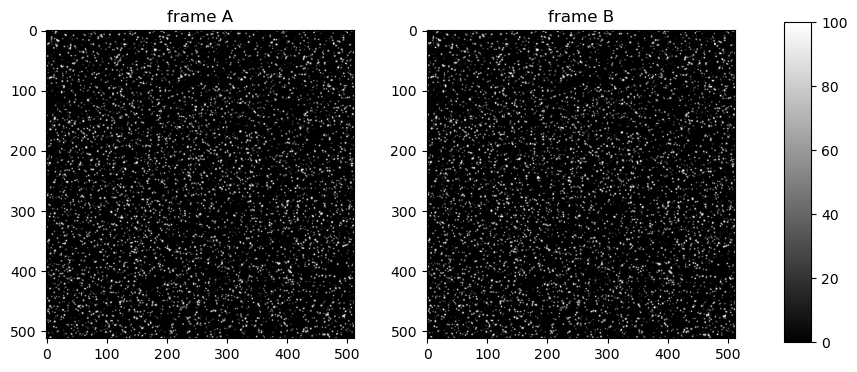
\includegraphics[keepaspectratio]{piv_basics_files/figure-pdf/cell-3-output-1.png}}

The two images show the particles at two different times. But these
images are way to big and contain too many particles to manually track
the movement of individual particles from one frame to the other.
Instead, we can analyze small regions of interest, called interrogation
windows (IW). Typically, we can start with a size of 32 x 32 pixels or
smaller. Until recently, the fast algorithms used powers of 2, so the
historical sizes are always powers of 2: 8, 16, 32, 64, 128, \ldots{}

Let's take the first top left windows from each image.

\begin{Shaded}
\begin{Highlighting}[]
\NormalTok{win\_size }\OperatorTok{=} \DecValTok{32}

\NormalTok{a\_win }\OperatorTok{=}\NormalTok{ a[:win\_size, :win\_size].copy()}
\NormalTok{b\_win }\OperatorTok{=}\NormalTok{ b[:win\_size, :win\_size].copy()}

\NormalTok{fig, axs }\OperatorTok{=}\NormalTok{ plt.subplots(}\DecValTok{1}\NormalTok{, }\DecValTok{2}\NormalTok{, figsize}\OperatorTok{=}\NormalTok{(}\DecValTok{9}\NormalTok{, }\DecValTok{4}\NormalTok{))}
\NormalTok{img }\OperatorTok{=}\NormalTok{ axs[}\DecValTok{0}\NormalTok{].imshow(a\_win, vmin}\OperatorTok{=}\DecValTok{0}\NormalTok{, vmax}\OperatorTok{=}\DecValTok{100}\NormalTok{, cmap}\OperatorTok{=}\NormalTok{plt.cm.gray)}
\NormalTok{axs[}\DecValTok{0}\NormalTok{].set\_title(}\StringTok{\textquotesingle{}IA\textquotesingle{}}\NormalTok{)}

\NormalTok{img }\OperatorTok{=}\NormalTok{ axs[}\DecValTok{1}\NormalTok{].imshow(b\_win, vmin}\OperatorTok{=}\DecValTok{0}\NormalTok{, vmax}\OperatorTok{=}\DecValTok{100}\NormalTok{, cmap}\OperatorTok{=}\NormalTok{plt.cm.gray)}
\NormalTok{axs[}\DecValTok{1}\NormalTok{].set\_title(}\StringTok{\textquotesingle{}IB\textquotesingle{}}\NormalTok{)}

\NormalTok{cbar }\OperatorTok{=}\NormalTok{ fig.add\_axes([}\FloatTok{0.95}\NormalTok{, }\FloatTok{0.1}\NormalTok{, }\FloatTok{0.03}\NormalTok{, }\FloatTok{0.8}\NormalTok{])}
\NormalTok{fig.colorbar(img, cax}\OperatorTok{=}\NormalTok{cbar)}
\NormalTok{plt.show()}
\end{Highlighting}
\end{Shaded}

\pandocbounded{\includegraphics[keepaspectratio]{piv_basics_files/figure-pdf/cell-4-output-1.png}}

If you tried to manually track the movement of individual particles from
frame A to frame B, it would be extremely time-consuming, especially for
large image regions containing many particles. Manually identifying and
matching every single particle would quickly become tedious and
impractical for even a coarse velocity field estimation. That's why
automated methods, such as using correlation techniques or least squares
approaches, are preferred in Particle Image Velocimetry (PIV). These
methods can efficiently analyze the displacement of all particles within
interrogation windows and generate a velocity field much faster and more
accurately than manual matching.

We can find out the distance that all the particles moved between frame
A and frame B using the principles of least squares or correlations, but
let's first try to get it manually.

If we try to shift the window IA by some pixels along the horizontal
and/or vertical directions, we shall see an image that gets closer in
resemblance to the window IB.

\textbf{Assignment:} Modify the code below to minimize the difference
between the shifted IA and IB.

\begin{Shaded}
\begin{Highlighting}[]
\NormalTok{fig, axs }\OperatorTok{=}\NormalTok{ plt.subplots(}\DecValTok{1}\NormalTok{, }\DecValTok{3}\NormalTok{, figsize}\OperatorTok{=}\NormalTok{(}\DecValTok{9}\NormalTok{, }\DecValTok{4}\NormalTok{))}

\NormalTok{img }\OperatorTok{=}\NormalTok{ axs[}\DecValTok{0}\NormalTok{].imshow(a\_win, cmap}\OperatorTok{=}\NormalTok{plt.cm.gray)}
\NormalTok{axs[}\DecValTok{0}\NormalTok{].set\_title(}\StringTok{"IA(shift=0)"}\NormalTok{)}

\NormalTok{img }\OperatorTok{=}\NormalTok{ axs[}\DecValTok{1}\NormalTok{].imshow(np.roll(a\_win, (}\DecValTok{0}\NormalTok{, }\DecValTok{1}\NormalTok{), axis}\OperatorTok{=}\NormalTok{(}\DecValTok{0}\NormalTok{, }\DecValTok{1}\NormalTok{)), cmap}\OperatorTok{=}\NormalTok{plt.cm.gray)}
\NormalTok{axs[}\DecValTok{1}\NormalTok{].set\_title(}\StringTok{"IA(shift=1 pxl)"}\NormalTok{)}

\NormalTok{img }\OperatorTok{=}\NormalTok{ axs[}\DecValTok{2}\NormalTok{].imshow(b\_win, cmap}\OperatorTok{=}\NormalTok{plt.cm.gray)}
\NormalTok{axs[}\DecValTok{2}\NormalTok{].set\_title(}\StringTok{"IB"}\NormalTok{)}

\NormalTok{cbar }\OperatorTok{=}\NormalTok{ fig.add\_axes([}\FloatTok{0.95}\NormalTok{, }\FloatTok{0.1}\NormalTok{, }\FloatTok{0.03}\NormalTok{, }\FloatTok{0.8}\NormalTok{])}
\NormalTok{fig.colorbar(img, cax}\OperatorTok{=}\NormalTok{cbar)}
\NormalTok{plt.show()}
\end{Highlighting}
\end{Shaded}

\pandocbounded{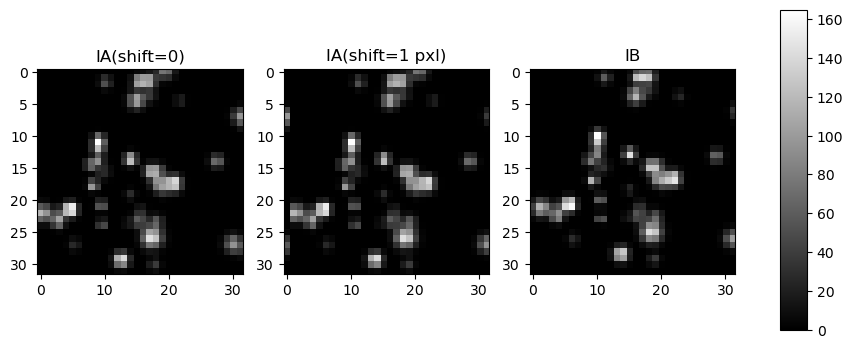
\includegraphics[keepaspectratio]{piv_basics_files/figure-pdf/cell-5-output-1.png}}

If we now subtract from IB the shifted IA, we shall see how good the
shift predicts the real displacement between the two.

\textbf{Assignment:} Modify the code below to minimize the difference
between the shifted IA and IB. Share your comments.

\begin{Shaded}
\begin{Highlighting}[]
\NormalTok{fig, axs }\OperatorTok{=}\NormalTok{ plt.subplots(}\DecValTok{1}\NormalTok{, }\DecValTok{3}\NormalTok{, figsize}\OperatorTok{=}\NormalTok{(}\DecValTok{9}\NormalTok{, }\DecValTok{4}\NormalTok{))}

\NormalTok{img }\OperatorTok{=}\NormalTok{ axs[}\DecValTok{0}\NormalTok{].imshow(b\_win }\OperatorTok{{-}}\NormalTok{ a\_win, cmap}\OperatorTok{=}\NormalTok{plt.cm.gray)}
\NormalTok{axs[}\DecValTok{0}\NormalTok{].set\_title(}\StringTok{"IB {-} IA(shift=0)"}\NormalTok{)}

\NormalTok{img }\OperatorTok{=}\NormalTok{ axs[}\DecValTok{1}\NormalTok{].imshow(b\_win }\OperatorTok{{-}}\NormalTok{ np.roll(a\_win, (}\DecValTok{1}\NormalTok{, }\DecValTok{0}\NormalTok{), axis}\OperatorTok{=}\NormalTok{(}\DecValTok{0}\NormalTok{, }\DecValTok{1}\NormalTok{)), cmap}\OperatorTok{=}\NormalTok{plt.cm.gray)}
\NormalTok{axs[}\DecValTok{1}\NormalTok{].set\_title(}\StringTok{"IB {-} IA(shift=1 pxl)"}\NormalTok{)}

\NormalTok{img }\OperatorTok{=}\NormalTok{ axs[}\DecValTok{2}\NormalTok{].imshow(b\_win }\OperatorTok{{-}}\NormalTok{ np.roll(a\_win, (}\DecValTok{2}\NormalTok{, }\DecValTok{0}\NormalTok{), axis}\OperatorTok{=}\NormalTok{(}\DecValTok{0}\NormalTok{, }\DecValTok{1}\NormalTok{)), cmap}\OperatorTok{=}\NormalTok{plt.cm.gray)}
\NormalTok{axs[}\DecValTok{2}\NormalTok{].set\_title(}\StringTok{"IB {-} IA(shift=2 pxl)"}\NormalTok{)}

\NormalTok{cbar }\OperatorTok{=}\NormalTok{ fig.add\_axes([}\FloatTok{0.95}\NormalTok{, }\FloatTok{0.1}\NormalTok{, }\FloatTok{0.03}\NormalTok{, }\FloatTok{0.8}\NormalTok{])}
\NormalTok{fig.colorbar(img, cax}\OperatorTok{=}\NormalTok{cbar)}
\NormalTok{plt.show()}
\end{Highlighting}
\end{Shaded}

\pandocbounded{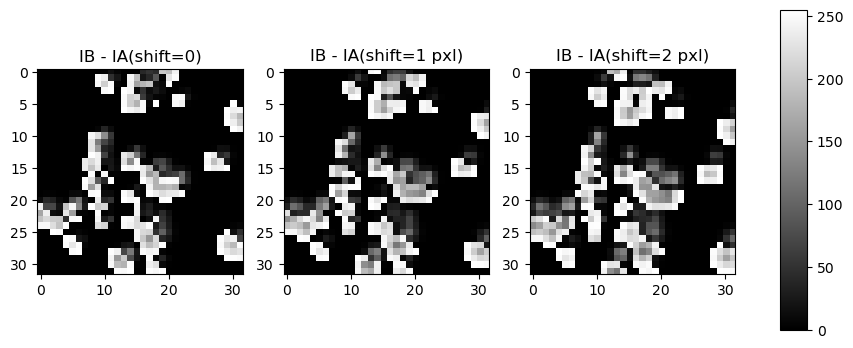
\includegraphics[keepaspectratio]{piv_basics_files/figure-pdf/cell-6-output-1.png}}

Let's try to find the best shift algorithmically: shift and calculate
the sum of squared differences, the minimum of which should be the best
shift.

\begin{Shaded}
\begin{Highlighting}[]
\KeywordTok{def}\NormalTok{ match\_template(img, template, maxroll}\OperatorTok{=}\DecValTok{8}\NormalTok{):}
    \CommentTok{\# img: input image to compare}
    \CommentTok{\# template: image to match against}
    \CommentTok{\# maxroll: max nbr of pxl to shift in each dir. Default value is 8.}
\NormalTok{    best\_dist }\OperatorTok{=}\NormalTok{ np.inf}
\NormalTok{    best\_shift }\OperatorTok{=}\NormalTok{ (}\OperatorTok{{-}}\DecValTok{1}\NormalTok{, }\OperatorTok{{-}}\DecValTok{1}\NormalTok{)}
    \ControlFlowTok{for}\NormalTok{ y }\KeywordTok{in} \BuiltInTok{range}\NormalTok{(}\OperatorTok{{-}}\NormalTok{maxroll,maxroll):}
        \ControlFlowTok{for}\NormalTok{ x }\KeywordTok{in} \BuiltInTok{range}\NormalTok{(}\OperatorTok{{-}}\NormalTok{maxroll,maxroll):}
            \CommentTok{\# calculate Euclidean distance}
\NormalTok{            dist }\OperatorTok{=}\NormalTok{ np.sqrt(np.}\BuiltInTok{sum}\NormalTok{((img }\OperatorTok{{-}}\NormalTok{ np.roll(template, (y, x), axis}\OperatorTok{=}\NormalTok{(}\DecValTok{0}\NormalTok{, }\DecValTok{1}\NormalTok{))) }\OperatorTok{**} \DecValTok{2}\NormalTok{))}
            \ControlFlowTok{if}\NormalTok{ dist }\OperatorTok{\textless{}}\NormalTok{ best\_dist:}
\NormalTok{                best\_dist }\OperatorTok{=}\NormalTok{ dist}
\NormalTok{                best\_shift }\OperatorTok{=}\NormalTok{ (y, x)}
    \ControlFlowTok{return}\NormalTok{ (best\_dist, best\_shift)}
\end{Highlighting}
\end{Shaded}

Let's check that it works by manually shifting the same image (IA):

\begin{Shaded}
\begin{Highlighting}[]
\NormalTok{match\_template(np.roll(a\_win, (}\DecValTok{2}\NormalTok{, }\DecValTok{0}\NormalTok{), axis}\OperatorTok{=}\NormalTok{(}\DecValTok{0}\NormalTok{, }\DecValTok{1}\NormalTok{)), a\_win)}
\end{Highlighting}
\end{Shaded}

\begin{verbatim}
(0.0, (2, 0))
\end{verbatim}

Indeed, when we find the correct shift, we get zero distance. It's not
so in real images:

\begin{Shaded}
\begin{Highlighting}[]
\NormalTok{match\_template(b\_win, a\_win)}
\end{Highlighting}
\end{Shaded}

\begin{verbatim}
(123.80226169178009, (-1, 1))
\end{verbatim}

Well, this is not the true displacement, but it gives a hint.

We could draw this as a vector of velocity

\[
    u = \frac{\Delta x \text{ pixels}}{\Delta t} ,\qquad v = \frac{\Delta y \text{ pixels}}{\Delta t}
\]

where \(\Delta t\) is the time interval (delay) between the two images
(or two laser pulses).

The problem is that shifting each image and repeating the loop many
times is impractical.

However, one can get it by using a different matching principle, based
on the property called cross-correlation (cross because we use two
different images). This is an efficient computational algorithm to find
out the right shift. You can see more details here:
http://paulbourke.net/miscellaneous/correlate/.

\begin{Shaded}
\begin{Highlighting}[]
\ImportTok{from}\NormalTok{ scipy.signal }\ImportTok{import}\NormalTok{ correlate}

\NormalTok{cross\_corr }\OperatorTok{=}\NormalTok{ correlate(b\_win }\OperatorTok{{-}}\NormalTok{ b\_win.mean(), a\_win }\OperatorTok{{-}}\NormalTok{ a\_win.mean(), method}\OperatorTok{=}\StringTok{"fft"}\NormalTok{)}
\CommentTok{\# Note that it\textquotesingle{}s approximately twice as large as the original windows, as we}
\CommentTok{\# can shift a\_win by a maximum of its size horizontally and vertically}
\CommentTok{\# while still maintaining some overlap between the two windows.}
\BuiltInTok{print}\NormalTok{(}\StringTok{"Size of the correlation map: }\SpecialCharTok{\%d}\StringTok{ x }\SpecialCharTok{\%d}\StringTok{"} \OperatorTok{\%}\NormalTok{ cross\_corr.shape)}
\end{Highlighting}
\end{Shaded}

\begin{verbatim}
Size of the correlation map: 63 x 63
\end{verbatim}

\begin{Shaded}
\begin{Highlighting}[]
\CommentTok{\# let\textquotesingle{}s see what the cross{-}correlation looks like}
\CommentTok{\#from mpl\_toolkits.mplot3d import Axes3D}
\NormalTok{Y, X }\OperatorTok{=}\NormalTok{ np.meshgrid(np.arange(cross\_corr.shape[}\DecValTok{0}\NormalTok{]), np.arange(cross\_corr.shape[}\DecValTok{1}\NormalTok{]))}

\NormalTok{fig }\OperatorTok{=}\NormalTok{ plt.figure()}
\NormalTok{ax }\OperatorTok{=}\NormalTok{ fig.add\_subplot(projection}\OperatorTok{=}\StringTok{"3d"}\NormalTok{)}
\NormalTok{ax.plot\_surface(Y, X, cross\_corr, cmap}\OperatorTok{=}\StringTok{\textquotesingle{}jet\textquotesingle{}}\NormalTok{, linewidth}\OperatorTok{=}\FloatTok{0.2}\NormalTok{)  }\CommentTok{\# type: ignore}
\NormalTok{plt.title(}\StringTok{"Correlation map — peak is the most probable shift"}\NormalTok{)}
\NormalTok{plt.show()}

\CommentTok{\# let\textquotesingle{}s see the same correlation map, from above}
\NormalTok{plt.imshow(cross\_corr, cmap}\OperatorTok{=}\NormalTok{plt.cm.gray)}
\NormalTok{y, x }\OperatorTok{=}\NormalTok{ np.unravel\_index(cross\_corr.argmax(), cross\_corr.shape)}
\BuiltInTok{print}\NormalTok{(}\SpecialStringTok{f"}\SpecialCharTok{\{}\NormalTok{y}\OperatorTok{=}\SpecialCharTok{\}}\SpecialStringTok{, }\SpecialCharTok{\{}\NormalTok{x}\OperatorTok{=}\SpecialCharTok{\}}\SpecialStringTok{"}\NormalTok{)}
\NormalTok{plt.plot(x, y, }\StringTok{"ro"}\NormalTok{)}
\NormalTok{plt.show()}
\end{Highlighting}
\end{Shaded}

\pandocbounded{\includegraphics[keepaspectratio]{piv_basics_files/figure-pdf/cell-11-output-1.png}}

\begin{verbatim}
y=30, x=32
\end{verbatim}

\pandocbounded{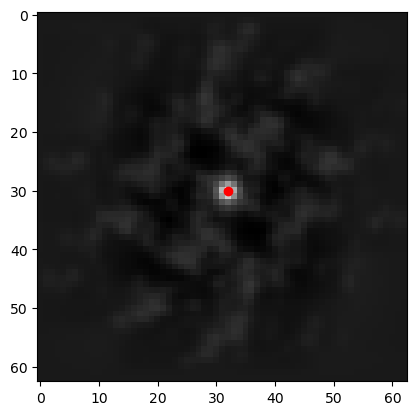
\includegraphics[keepaspectratio]{piv_basics_files/figure-pdf/cell-11-output-3.png}}

The image of the correlation map shows the same result that we got
manually looping. We need to substract the center of symmetry
\texttt{(31,\ 31)} to get the estimated displacement.

\begin{Shaded}
\begin{Highlighting}[]
\NormalTok{dy, dx }\OperatorTok{=}\NormalTok{ y }\OperatorTok{{-}} \DecValTok{31}\NormalTok{, x }\OperatorTok{{-}} \DecValTok{31}
\BuiltInTok{print}\NormalTok{(}\SpecialStringTok{f"}\SpecialCharTok{\{}\NormalTok{dy}\OperatorTok{=}\SpecialCharTok{\}}\SpecialStringTok{, }\SpecialCharTok{\{}\NormalTok{dx}\OperatorTok{=}\SpecialCharTok{\}}\SpecialStringTok{"}\NormalTok{)}
\end{Highlighting}
\end{Shaded}

\begin{verbatim}
dy=-1, dx=1
\end{verbatim}

We can get the first velocity field by repeating this analysis for all
small windows. Let's take 32 x 32 pixels windows from each image and do
the loop:

\begin{Shaded}
\begin{Highlighting}[]
\KeywordTok{def}\NormalTok{ vel\_field(curr\_frame, next\_frame, win\_size):}
\NormalTok{    ys }\OperatorTok{=}\NormalTok{ np.arange(}\DecValTok{0}\NormalTok{, curr\_frame.shape[}\DecValTok{0}\NormalTok{], win\_size)}
\NormalTok{    xs }\OperatorTok{=}\NormalTok{ np.arange(}\DecValTok{0}\NormalTok{, curr\_frame.shape[}\DecValTok{1}\NormalTok{], win\_size)}
\NormalTok{    dys }\OperatorTok{=}\NormalTok{ np.zeros((}\BuiltInTok{len}\NormalTok{(ys), }\BuiltInTok{len}\NormalTok{(xs)))}
\NormalTok{    dxs }\OperatorTok{=}\NormalTok{ np.zeros((}\BuiltInTok{len}\NormalTok{(ys), }\BuiltInTok{len}\NormalTok{(xs)))}
    \ControlFlowTok{for}\NormalTok{ iy, y }\KeywordTok{in} \BuiltInTok{enumerate}\NormalTok{(ys):}
        \ControlFlowTok{for}\NormalTok{ ix, x }\KeywordTok{in} \BuiltInTok{enumerate}\NormalTok{(xs):}
\NormalTok{            int\_win }\OperatorTok{=}\NormalTok{ curr\_frame[y : y }\OperatorTok{+}\NormalTok{ win\_size, x : x }\OperatorTok{+}\NormalTok{ win\_size]}
\NormalTok{            search\_win }\OperatorTok{=}\NormalTok{ next\_frame[y : y }\OperatorTok{+}\NormalTok{ win\_size, x : x }\OperatorTok{+}\NormalTok{ win\_size]}
\NormalTok{            cross\_corr }\OperatorTok{=}\NormalTok{ correlate(}
\NormalTok{                search\_win }\OperatorTok{{-}}\NormalTok{ search\_win.mean(), int\_win }\OperatorTok{{-}}\NormalTok{ int\_win.mean(), method}\OperatorTok{=}\StringTok{"fft"}
\NormalTok{            )}
\NormalTok{            dys[iy, ix], dxs[iy, ix] }\OperatorTok{=}\NormalTok{ (}
\NormalTok{                np.unravel\_index(np.argmax(cross\_corr), cross\_corr.shape)}
                \OperatorTok{{-}}\NormalTok{ np.array([win\_size, win\_size])}
                \OperatorTok{+} \DecValTok{1}
\NormalTok{            )}
    \CommentTok{\# draw velocity vectors from the center of each window}
\NormalTok{    ys }\OperatorTok{=}\NormalTok{ ys }\OperatorTok{+}\NormalTok{ win\_size }\OperatorTok{/} \DecValTok{2}
\NormalTok{    xs }\OperatorTok{=}\NormalTok{ xs }\OperatorTok{+}\NormalTok{ win\_size }\OperatorTok{/} \DecValTok{2}
    \ControlFlowTok{return}\NormalTok{ xs, ys, dxs, dys}
\end{Highlighting}
\end{Shaded}

\begin{Shaded}
\begin{Highlighting}[]
\NormalTok{xs, ys, dxs, dys }\OperatorTok{=}\NormalTok{ vel\_field(a, b, }\DecValTok{32}\NormalTok{)}
\NormalTok{norm\_drs }\OperatorTok{=}\NormalTok{ np.sqrt(dxs }\OperatorTok{**} \DecValTok{2} \OperatorTok{+}\NormalTok{ dys }\OperatorTok{**} \DecValTok{2}\NormalTok{)}

\NormalTok{fig, ax }\OperatorTok{=}\NormalTok{ plt.subplots(figsize}\OperatorTok{=}\NormalTok{(}\DecValTok{9}\NormalTok{, }\DecValTok{4}\NormalTok{))}
\CommentTok{\# we need these flips on y since quiver uses a bottom{-}left origin, while our}
\CommentTok{\# arrays use a top{-}right origin}
\NormalTok{ax.quiver(}
\NormalTok{    xs,}
\NormalTok{    ys[::}\OperatorTok{{-}}\DecValTok{1}\NormalTok{],}
\NormalTok{    dxs,}
    \OperatorTok{{-}}\NormalTok{dys,}
\NormalTok{    norm\_drs,}
\NormalTok{    cmap}\OperatorTok{=}\StringTok{"plasma"}\NormalTok{,}
\NormalTok{    angles}\OperatorTok{=}\StringTok{"xy"}\NormalTok{,}
\NormalTok{    scale\_units}\OperatorTok{=}\StringTok{"xy"}\NormalTok{,}
\NormalTok{    scale}\OperatorTok{=}\FloatTok{0.25}\NormalTok{,}
\NormalTok{)}
\NormalTok{ax.set\_aspect(}\StringTok{"equal"}\NormalTok{)}
\NormalTok{plt.show()}
\end{Highlighting}
\end{Shaded}

\pandocbounded{\includegraphics[keepaspectratio]{piv_basics_files/figure-pdf/cell-14-output-1.png}}

If you've followed along this far, great! Now you understand the basics.

We can also try out a variant of this that uses a search window larger
than the interrogation window instead of relying on zero-padding. By
avoiding using zero-padding around the search window, movement detection
should theoretically be a bit better, assuming that the window sizes are
chosen well.

\begin{Shaded}
\begin{Highlighting}[]
\KeywordTok{def}\NormalTok{ vel\_field\_asymmetric\_wins(}
\NormalTok{    curr\_frame, next\_frame, half\_int\_win\_size, half\_search\_win\_size}
\NormalTok{):}
\NormalTok{    ys }\OperatorTok{=}\NormalTok{ np.arange(half\_int\_win\_size[}\DecValTok{0}\NormalTok{], curr\_frame.shape[}\DecValTok{0}\NormalTok{], }\DecValTok{2} \OperatorTok{*}\NormalTok{ half\_int\_win\_size[}\DecValTok{0}\NormalTok{])}
\NormalTok{    xs }\OperatorTok{=}\NormalTok{ np.arange(half\_int\_win\_size[}\DecValTok{1}\NormalTok{], curr\_frame.shape[}\DecValTok{1}\NormalTok{], }\DecValTok{2} \OperatorTok{*}\NormalTok{ half\_int\_win\_size[}\DecValTok{1}\NormalTok{])}
\NormalTok{    dys }\OperatorTok{=}\NormalTok{ np.zeros((}\BuiltInTok{len}\NormalTok{(ys), }\BuiltInTok{len}\NormalTok{(xs)))}
\NormalTok{    dxs }\OperatorTok{=}\NormalTok{ np.zeros((}\BuiltInTok{len}\NormalTok{(ys), }\BuiltInTok{len}\NormalTok{(xs)))}
    \ControlFlowTok{for}\NormalTok{ iy, y }\KeywordTok{in} \BuiltInTok{enumerate}\NormalTok{(ys):}
        \ControlFlowTok{for}\NormalTok{ ix, x }\KeywordTok{in} \BuiltInTok{enumerate}\NormalTok{(xs):}
\NormalTok{            int\_win }\OperatorTok{=}\NormalTok{ curr\_frame[}
\NormalTok{                y }\OperatorTok{{-}}\NormalTok{ half\_int\_win\_size[}\DecValTok{0}\NormalTok{] : y }\OperatorTok{+}\NormalTok{ half\_int\_win\_size[}\DecValTok{0}\NormalTok{],}
\NormalTok{                x }\OperatorTok{{-}}\NormalTok{ half\_int\_win\_size[}\DecValTok{1}\NormalTok{] : x }\OperatorTok{+}\NormalTok{ half\_int\_win\_size[}\DecValTok{1}\NormalTok{],}
\NormalTok{            ]}
\NormalTok{            search\_win\_y\_min }\OperatorTok{=}\NormalTok{ y }\OperatorTok{{-}}\NormalTok{ half\_search\_win\_size[}\DecValTok{0}\NormalTok{]}
\NormalTok{            search\_win\_y\_max }\OperatorTok{=}\NormalTok{ y }\OperatorTok{+}\NormalTok{ half\_search\_win\_size[}\DecValTok{0}\NormalTok{]}
\NormalTok{            search\_win\_x\_min }\OperatorTok{=}\NormalTok{ x }\OperatorTok{{-}}\NormalTok{ half\_search\_win\_size[}\DecValTok{1}\NormalTok{]}
\NormalTok{            search\_win\_x\_max }\OperatorTok{=}\NormalTok{ x }\OperatorTok{+}\NormalTok{ half\_search\_win\_size[}\DecValTok{1}\NormalTok{]}
\NormalTok{            truncated\_search\_win }\OperatorTok{=}\NormalTok{ next\_frame[}
                \BuiltInTok{max}\NormalTok{(}\DecValTok{0}\NormalTok{, search\_win\_y\_min) : }\BuiltInTok{min}\NormalTok{(b.shape[}\DecValTok{0}\NormalTok{], search\_win\_y\_max),}
                \BuiltInTok{max}\NormalTok{(}\DecValTok{0}\NormalTok{, search\_win\_x\_min) : }\BuiltInTok{min}\NormalTok{(b.shape[}\DecValTok{1}\NormalTok{], search\_win\_x\_max),}
\NormalTok{            ]}
\NormalTok{            cross\_corr }\OperatorTok{=}\NormalTok{ correlate(}
\NormalTok{                truncated\_search\_win }\OperatorTok{{-}}\NormalTok{ np.mean(truncated\_search\_win),}
\NormalTok{                int\_win }\OperatorTok{{-}}\NormalTok{ np.mean(int\_win),}
\NormalTok{                mode}\OperatorTok{=}\StringTok{"valid"}\NormalTok{,}
\NormalTok{                method}\OperatorTok{=}\StringTok{"fft"}\NormalTok{,}
\NormalTok{            )}
\NormalTok{            dy, dx }\OperatorTok{=}\NormalTok{ np.unravel\_index(np.argmax(cross\_corr), cross\_corr.shape)}
            \CommentTok{\# if the top of the search window got truncated, shift the origin}
            \CommentTok{\# up to the top edge of the (non{-}truncated) search window}
            \ControlFlowTok{if}\NormalTok{ search\_win\_y\_min }\OperatorTok{\textless{}} \DecValTok{0}\NormalTok{:}
\NormalTok{                dy }\OperatorTok{+=} \OperatorTok{{-}}\NormalTok{search\_win\_y\_min}
            \CommentTok{\# if the left of the search window got truncated, shift the origin}
            \CommentTok{\# over to the left edge of the (non{-}truncated) search window}
            \ControlFlowTok{if}\NormalTok{ search\_win\_x\_min }\OperatorTok{\textless{}} \DecValTok{0}\NormalTok{:}
\NormalTok{                dx }\OperatorTok{+=} \OperatorTok{{-}}\NormalTok{search\_win\_x\_min}
            \CommentTok{\# shift origin to the center of the search window}
\NormalTok{            dy }\OperatorTok{{-}=}\NormalTok{ half\_search\_win\_size[}\DecValTok{0}\NormalTok{] }\OperatorTok{{-}}\NormalTok{ half\_int\_win\_size[}\DecValTok{0}\NormalTok{]}
\NormalTok{            dx }\OperatorTok{{-}=}\NormalTok{ half\_search\_win\_size[}\DecValTok{1}\NormalTok{] }\OperatorTok{{-}}\NormalTok{ half\_int\_win\_size[}\DecValTok{1}\NormalTok{]}
\NormalTok{            dys[iy, ix] }\OperatorTok{=}\NormalTok{ dy}
\NormalTok{            dxs[iy, ix] }\OperatorTok{=}\NormalTok{ dx}
    \ControlFlowTok{return}\NormalTok{ xs, ys, dxs, dys}
\end{Highlighting}
\end{Shaded}

\begin{Shaded}
\begin{Highlighting}[]
\NormalTok{int\_win\_size }\OperatorTok{=}\NormalTok{ np.array([}\DecValTok{32}\NormalTok{, }\DecValTok{32}\NormalTok{])}
\BuiltInTok{print}\NormalTok{(}\SpecialStringTok{f"}\SpecialCharTok{\{}\NormalTok{int\_win\_size}\OperatorTok{=}\SpecialCharTok{\}}\SpecialStringTok{"}\NormalTok{)}
\ControlFlowTok{assert}\NormalTok{ np.}\BuiltInTok{all}\NormalTok{(np.array(a.shape) }\OperatorTok{\%}\NormalTok{ int\_win\_size }\OperatorTok{==} \DecValTok{0}\NormalTok{)}
\ControlFlowTok{assert}\NormalTok{ np.}\BuiltInTok{all}\NormalTok{(int\_win\_size }\OperatorTok{\%} \DecValTok{2} \OperatorTok{==} \DecValTok{0}\NormalTok{)}
\NormalTok{half\_int\_win\_size }\OperatorTok{=}\NormalTok{ int\_win\_size }\OperatorTok{//} \DecValTok{2}

\NormalTok{search\_win\_size }\OperatorTok{=}\NormalTok{ int\_win\_size }\OperatorTok{*} \DecValTok{2}
\BuiltInTok{print}\NormalTok{(}\SpecialStringTok{f"}\SpecialCharTok{\{}\NormalTok{search\_win\_size}\OperatorTok{=}\SpecialCharTok{\}}\SpecialStringTok{"}\NormalTok{)}
\ControlFlowTok{assert}\NormalTok{ np.}\BuiltInTok{all}\NormalTok{(search\_win\_size }\OperatorTok{\%} \DecValTok{2} \OperatorTok{==} \DecValTok{0}\NormalTok{)}
\NormalTok{half\_search\_win\_size }\OperatorTok{=}\NormalTok{ search\_win\_size }\OperatorTok{//} \DecValTok{2}
\ControlFlowTok{assert}\NormalTok{ np.}\BuiltInTok{all}\NormalTok{(search\_win\_size }\OperatorTok{\textgreater{}}\NormalTok{ int\_win\_size)}
\BuiltInTok{print}\NormalTok{(}
    \StringTok{"max velocity that can be detected with these window sizes: "}
    \OperatorTok{+} \SpecialStringTok{f"}\SpecialCharTok{\{}\NormalTok{half\_search\_win\_size }\OperatorTok{{-}}\NormalTok{ half\_int\_win\_size}\SpecialCharTok{\}}\SpecialStringTok{"}
\NormalTok{)}
\end{Highlighting}
\end{Shaded}

\begin{verbatim}
int_win_size=array([32, 32])
search_win_size=array([64, 64])
max velocity that can be detected with these window sizes: [16 16]
\end{verbatim}

Making the search window larger compared to the interrogation window
would allow for larger velocities to be detected.

\begin{Shaded}
\begin{Highlighting}[]
\NormalTok{xs\_asym, ys\_asym, dxs\_asym, dys\_asym }\OperatorTok{=}\NormalTok{ vel\_field\_asymmetric\_wins(}
\NormalTok{    a, b, half\_int\_win\_size, half\_search\_win\_size}
\NormalTok{)}
\NormalTok{norm\_drs\_asym }\OperatorTok{=}\NormalTok{ np.sqrt(dxs\_asym }\OperatorTok{**} \DecValTok{2} \OperatorTok{+}\NormalTok{ dys\_asym }\OperatorTok{**} \DecValTok{2}\NormalTok{)}

\NormalTok{fig, axs }\OperatorTok{=}\NormalTok{ plt.subplots(}\DecValTok{1}\NormalTok{, }\DecValTok{2}\NormalTok{, figsize}\OperatorTok{=}\NormalTok{(}\DecValTok{9}\NormalTok{, }\DecValTok{4}\NormalTok{))}
\NormalTok{axs[}\DecValTok{0}\NormalTok{].quiver(}
\NormalTok{    xs,}
\NormalTok{    ys[::}\OperatorTok{{-}}\DecValTok{1}\NormalTok{],}
\NormalTok{    dxs,}
    \OperatorTok{{-}}\NormalTok{dys,}
\NormalTok{    norm\_drs,}
\NormalTok{    cmap}\OperatorTok{=}\StringTok{"plasma"}\NormalTok{,}
\NormalTok{    angles}\OperatorTok{=}\StringTok{"xy"}\NormalTok{,}
\NormalTok{    scale\_units}\OperatorTok{=}\StringTok{"xy"}\NormalTok{,}
\NormalTok{    scale}\OperatorTok{=}\FloatTok{0.25}\NormalTok{,}
\NormalTok{)}
\NormalTok{axs[}\DecValTok{1}\NormalTok{].quiver(}
\NormalTok{    xs\_asym,}
\NormalTok{    ys\_asym[::}\OperatorTok{{-}}\DecValTok{1}\NormalTok{],}
\NormalTok{    dxs\_asym,}
    \OperatorTok{{-}}\NormalTok{dys\_asym,}
\NormalTok{    norm\_drs\_asym,}
\NormalTok{    cmap}\OperatorTok{=}\StringTok{"plasma"}\NormalTok{,}
\NormalTok{    angles}\OperatorTok{=}\StringTok{"xy"}\NormalTok{,}
\NormalTok{    scale\_units}\OperatorTok{=}\StringTok{"xy"}\NormalTok{,}
\NormalTok{    scale}\OperatorTok{=}\FloatTok{0.25}\NormalTok{,}
\NormalTok{)}
\NormalTok{axs[}\DecValTok{0}\NormalTok{].set\_title(}
    \SpecialStringTok{f"}\SpecialCharTok{\{}\NormalTok{win\_size}\SpecialCharTok{\}}\SpecialStringTok{ x }\SpecialCharTok{\{}\NormalTok{win\_size}\SpecialCharTok{\}}\SpecialStringTok{ int. win. + "}
    \SpecialStringTok{f"}\SpecialCharTok{\{}\NormalTok{win\_size}\SpecialCharTok{\}}\SpecialStringTok{ x }\SpecialCharTok{\{}\NormalTok{win\_size}\SpecialCharTok{\}}\SpecialStringTok{ 0{-}padded search win."}
\NormalTok{)}
\NormalTok{axs[}\DecValTok{1}\NormalTok{].set\_title(}
    \SpecialStringTok{f"}\SpecialCharTok{\{}\NormalTok{int\_win\_size[}\DecValTok{0}\NormalTok{]}\SpecialCharTok{\}}\SpecialStringTok{ x }\SpecialCharTok{\{}\NormalTok{int\_win\_size[}\DecValTok{1}\NormalTok{]}\SpecialCharTok{\}}\SpecialStringTok{ int. win. + "}
    \SpecialStringTok{f"}\SpecialCharTok{\{}\NormalTok{search\_win\_size[}\DecValTok{0}\NormalTok{]}\SpecialCharTok{\}}\SpecialStringTok{ x }\SpecialCharTok{\{}\NormalTok{search\_win\_size[}\DecValTok{0}\NormalTok{]}\SpecialCharTok{\}}\SpecialStringTok{ unpadded search win."}
\NormalTok{)}
\NormalTok{ax.set\_aspect(}\StringTok{"equal"}\NormalTok{)}
\NormalTok{plt.show()}
\end{Highlighting}
\end{Shaded}

\pandocbounded{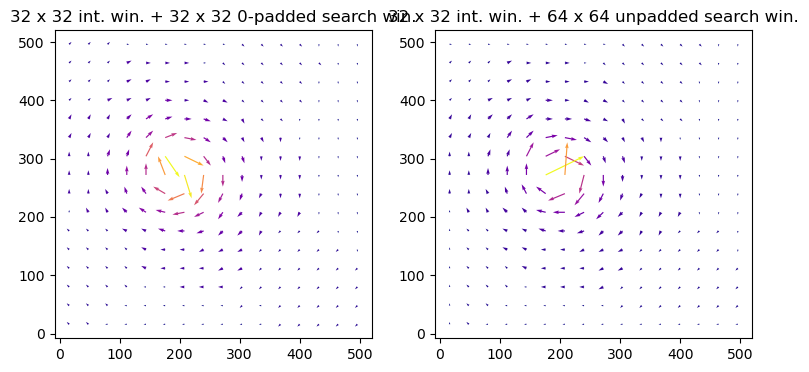
\includegraphics[keepaspectratio]{piv_basics_files/figure-pdf/cell-17-output-1.png}}

\chapter{OpenPIV first tutorial}\label{openpiv-first-tutorial}

Using open source software, OpenPIV (http://www.openpiv.net), written
with Python, Numpy, Scipy (http://www.scipy.org), we will introduce the
basics of PIV.

This tutorial will follow the simplest analysis path from the two images
to the velocity field and some post-analysis.

\begin{Shaded}
\begin{Highlighting}[]
\CommentTok{\# import the standard numerical and plotting packages}
\ImportTok{import}\NormalTok{ numpy }\ImportTok{as}\NormalTok{ np}
\ImportTok{import}\NormalTok{ matplotlib.pyplot }\ImportTok{as}\NormalTok{ plt}
\OperatorTok{\%}\NormalTok{matplotlib inline}
\CommentTok{\# import what is necessary from OpenPIV}
\ImportTok{from}\NormalTok{ openpiv }\ImportTok{import}\NormalTok{ tools, pyprocess, validation, filters, scaling}
\end{Highlighting}
\end{Shaded}

\begin{Shaded}
\begin{Highlighting}[]
\CommentTok{\# read a pair of PIV images}
\NormalTok{frame\_a  }\OperatorTok{=}\NormalTok{ tools.imread( }\StringTok{\textquotesingle{}./images/exp1\_001\_b.bmp\textquotesingle{}}\NormalTok{ )}
\NormalTok{frame\_b  }\OperatorTok{=}\NormalTok{ tools.imread( }\StringTok{\textquotesingle{}./images/exp1\_001\_c.bmp\textquotesingle{}}\NormalTok{ )}
\end{Highlighting}
\end{Shaded}

\begin{Shaded}
\begin{Highlighting}[]
\CommentTok{\# let\textquotesingle{}s visualize them using matplotlib}
\NormalTok{fig,ax }\OperatorTok{=}\NormalTok{ plt.subplots(}\DecValTok{1}\NormalTok{,}\DecValTok{2}\NormalTok{,figsize}\OperatorTok{=}\NormalTok{(}\DecValTok{10}\NormalTok{,}\DecValTok{8}\NormalTok{))}
\NormalTok{ax[}\DecValTok{0}\NormalTok{].imshow(frame\_a,cmap}\OperatorTok{=}\NormalTok{plt.cm.gray)}
\NormalTok{ax[}\DecValTok{1}\NormalTok{].imshow(frame\_b,cmap}\OperatorTok{=}\NormalTok{plt.cm.gray)}
\NormalTok{plt.show()}
\end{Highlighting}
\end{Shaded}

\pandocbounded{\includegraphics[keepaspectratio]{tutorial_files/figure-pdf/cell-4-output-1.png}}

\section{Processing}\label{processing}

We are going to use the \texttt{extended\_search\_area\_piv\ function},
wich is a standard PIV cross-correlation algorithm.

This function allows the search area (\texttt{search\_area\_size}) in
the second frame to be larger than the interrogation window in the first
frame (\texttt{window\_size}). Also, the search areas can overlap
(\texttt{overlap}).

The \texttt{extended\_search\_area\_piv} function will return three
arrays: 1. The \texttt{u} component of the velocity field 2. The
\texttt{v} component of the velocity field 3. The signal-to-noise ratio
(\texttt{sig2noise}) of the cross-correlation map of each vector. The
higher the signal-to-noise ratio, the higher the probability that its
magnitude and direction are correct.

\begin{Shaded}
\begin{Highlighting}[]
\CommentTok{\# define the PIV analysis parameters}
\NormalTok{winsize }\OperatorTok{=} \DecValTok{24} \CommentTok{\# size of the interrogation window in frame A, in pixels}
\NormalTok{searchsize }\OperatorTok{=} \DecValTok{32}  \CommentTok{\# size of the window in frame B (searchsize is larger or equal to winsize), in pixels}
\NormalTok{overlap }\OperatorTok{=} \DecValTok{12} \CommentTok{\# overlap between the neighbouring windows, in pixels}
\NormalTok{dt }\OperatorTok{=} \FloatTok{0.02} \CommentTok{\# time interval of the PIV recording, in sec}
\end{Highlighting}
\end{Shaded}

\begin{Shaded}
\begin{Highlighting}[]
\NormalTok{u, v, sig2noise }\OperatorTok{=}\NormalTok{ pyprocess.extended\_search\_area\_piv(}
\NormalTok{    frame\_a.astype(np.int32),}
\NormalTok{    frame\_b.astype(np.int32),}
\NormalTok{    window\_size}\OperatorTok{=}\NormalTok{winsize,}
\NormalTok{    overlap}\OperatorTok{=}\NormalTok{overlap,}
\NormalTok{    dt}\OperatorTok{=}\NormalTok{dt,}
\NormalTok{    search\_area\_size}\OperatorTok{=}\NormalTok{searchsize,}
\NormalTok{    sig2noise\_method}\OperatorTok{=}\StringTok{\textquotesingle{}peak2peak\textquotesingle{}}\NormalTok{,}
\NormalTok{)}
\end{Highlighting}
\end{Shaded}

The function \texttt{get\_coordinates} finds the center of each
interrogation window. This will be useful later on when plotting the
vector field.

\begin{Shaded}
\begin{Highlighting}[]
\CommentTok{\# get a list of coordinates for the vector field}
\NormalTok{x, y }\OperatorTok{=}\NormalTok{ pyprocess.get\_coordinates(}
\NormalTok{    image\_size}\OperatorTok{=}\NormalTok{frame\_a.shape,}
\NormalTok{    search\_area\_size}\OperatorTok{=}\NormalTok{searchsize,}
\NormalTok{    overlap}\OperatorTok{=}\NormalTok{overlap,}
\NormalTok{)}
\end{Highlighting}
\end{Shaded}

\section{Post-processing}\label{post-processing}

Strictly speaking, we are ready to plot the vector field. However, some
spurious vectors might locally impact the quality of the results. It
might therefore be useful to apply some filtering.

To start, let's use the function \texttt{sig2noise\_val} to get a mask
indicating which vectors have a minimum amount of signal-to-noise ratio.
Vectors below a certain threshold are substituted by \texttt{NaN}. If
you are not sure about which threshold value to use, try taking a look
at the signal-to-noise ratio histogram with:
\texttt{plt.hist(sig2noise.flatten())}.

\begin{Shaded}
\begin{Highlighting}[]
\CommentTok{\# clean the peaks that are below a quality threshold}
\NormalTok{invalid\_mask }\OperatorTok{=}\NormalTok{ validation.sig2noise\_val(}
\NormalTok{    sig2noise,}
\NormalTok{    threshold }\OperatorTok{=} \FloatTok{1.3}\NormalTok{,}
\NormalTok{)}
\end{Highlighting}
\end{Shaded}

Another useful function is \texttt{replace\_outliers}, which will find
outlier vectors and substitute them with an average of neighboring
vectors. The larger the \texttt{kernel\_size}, the larger the considered
neighborhood. This function uses an iterative image inpainting
algorithm. The number of iterations can be chosen via
\texttt{max\_iter}.

\begin{Shaded}
\begin{Highlighting}[]
\CommentTok{\# replace those that are masked as bad vectors with local interpolation}
\NormalTok{u, v }\OperatorTok{=}\NormalTok{ filters.replace\_outliers(}
\NormalTok{    u, v,}
\NormalTok{    invalid\_mask,}
\NormalTok{    method}\OperatorTok{=}\StringTok{\textquotesingle{}localmean\textquotesingle{}}\NormalTok{,}
\NormalTok{    max\_iter}\OperatorTok{=}\DecValTok{3}\NormalTok{,}
\NormalTok{    kernel\_size}\OperatorTok{=}\DecValTok{3}\NormalTok{,}
\NormalTok{)}
\end{Highlighting}
\end{Shaded}

Next, we are going to convert pixels to millimeters.

\begin{Shaded}
\begin{Highlighting}[]
\CommentTok{\# scale the results from pix/dt to mm/sec}
\NormalTok{x, y, u, v }\OperatorTok{=}\NormalTok{ scaling.uniform(x, y, u, v, scaling\_factor }\OperatorTok{=} \FloatTok{96.52}\NormalTok{ ) }\CommentTok{\# 96.52 pixels/millimeter}
\end{Highlighting}
\end{Shaded}

\section{Plot and save the results}\label{plot-and-save-the-results}

The vector field can be plotted with \texttt{display\_vector\_field}.
Vectors with signal-to-noise ratio below the threshold are displayed in
red.

\begin{Shaded}
\begin{Highlighting}[]
\ImportTok{import}\NormalTok{ pathlib}

\NormalTok{fig, ax }\OperatorTok{=}\NormalTok{ plt.subplots(figsize}\OperatorTok{=}\NormalTok{(}\DecValTok{9}\NormalTok{,}\DecValTok{4}\NormalTok{))}
\NormalTok{tools.display\_vector\_field(}
\NormalTok{    pathlib.Path(}\StringTok{\textquotesingle{}exp1\_001.txt\textquotesingle{}}\NormalTok{),}
\NormalTok{    ax}\OperatorTok{=}\NormalTok{ax, scaling\_factor}\OperatorTok{=}\FloatTok{96.52}\NormalTok{,}
\NormalTok{    scale}\OperatorTok{=}\DecValTok{50}\NormalTok{, }\CommentTok{\# scale defines here the arrow length}
\NormalTok{    width}\OperatorTok{=}\FloatTok{0.0035}\NormalTok{, }\CommentTok{\# width is the thickness of the arrow}
\NormalTok{    on\_img}\OperatorTok{=}\VariableTok{True}\NormalTok{, }\CommentTok{\# overlay on the image}
\NormalTok{    image\_name}\OperatorTok{=} \BuiltInTok{str}\NormalTok{(}\StringTok{\textquotesingle{}./images/exp1\_001\_b.bmp\textquotesingle{}}\NormalTok{),}
\NormalTok{)}
\NormalTok{plt.show()}
\end{Highlighting}
\end{Shaded}

\pandocbounded{\includegraphics[keepaspectratio]{tutorial_files/figure-pdf/cell-11-output-1.png}}

The function \texttt{save} is used to save the vector field to a ASCII
tabular file.

\begin{Shaded}
\begin{Highlighting}[]
\NormalTok{tools.save(}\StringTok{\textquotesingle{}exp1\_001.txt\textquotesingle{}}\NormalTok{ , x, y, u, v, invalid\_mask)}
\end{Highlighting}
\end{Shaded}

\chapter{Another example}\label{another-example}

\section{Use any pair of images that you can access via
URL}\label{use-any-pair-of-images-that-you-can-access-via-url}

For instance we can use images from PIV Challenge
http://www.pivchallenge.org/

\begin{Shaded}
\begin{Highlighting}[]
\NormalTok{frame\_a }\OperatorTok{=}\NormalTok{ tools.imread(}\StringTok{\textquotesingle{}http://www.pivchallenge.org/pub/B/B001\_1.tif\textquotesingle{}}\NormalTok{)}
\NormalTok{frame\_b }\OperatorTok{=}\NormalTok{ tools.imread(}\StringTok{\textquotesingle{}http://www.pivchallenge.org/pub/B/B001\_2.tif\textquotesingle{}}\NormalTok{)}
\CommentTok{\#frame\_a = tools.imread("./images/B005\_1.tif")}
\CommentTok{\#frame\_b = tools.imread("./images/B005\_2.tif")}
\NormalTok{fig,ax }\OperatorTok{=}\NormalTok{ plt.subplots(}\DecValTok{1}\NormalTok{,}\DecValTok{2}\NormalTok{,figsize}\OperatorTok{=}\NormalTok{(}\DecValTok{10}\NormalTok{,}\DecValTok{8}\NormalTok{))}
\NormalTok{ax[}\DecValTok{0}\NormalTok{].imshow(frame\_a,cmap}\OperatorTok{=}\NormalTok{plt.cm.gray)}
\NormalTok{ax[}\DecValTok{1}\NormalTok{].imshow(frame\_b,cmap}\OperatorTok{=}\NormalTok{plt.cm.gray)}
\NormalTok{plt.show()}
\end{Highlighting}
\end{Shaded}

\pandocbounded{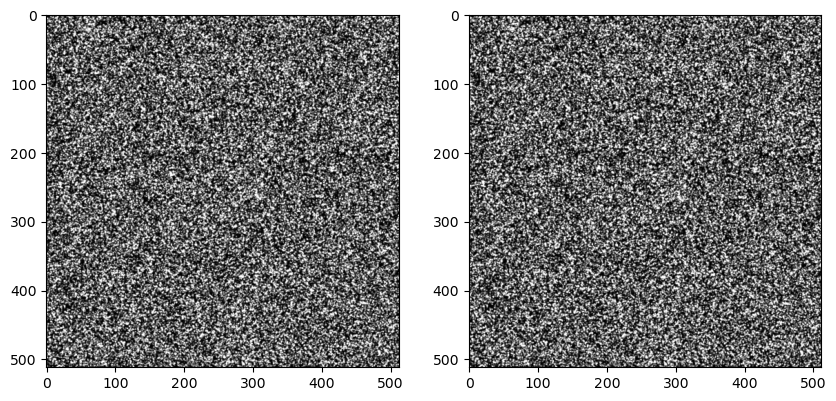
\includegraphics[keepaspectratio]{tutorial_files/figure-pdf/cell-13-output-1.png}}

\begin{Shaded}
\begin{Highlighting}[]
\NormalTok{winsize }\OperatorTok{=} \DecValTok{32} \CommentTok{\# pixels}
\NormalTok{searchsize }\OperatorTok{=} \DecValTok{64}  \CommentTok{\# pixels, search in image B}
\NormalTok{overlap }\OperatorTok{=} \DecValTok{16} \CommentTok{\# pixels}
\NormalTok{dt }\OperatorTok{=} \FloatTok{1.0} \CommentTok{\# sec}
\NormalTok{u, v, sig2noise }\OperatorTok{=}\NormalTok{ pyprocess.extended\_search\_area\_piv( frame\_a.astype(np.int32), frame\_b.astype(np.int32), window\_size}\OperatorTok{=}\NormalTok{winsize, overlap}\OperatorTok{=}\NormalTok{overlap, dt}\OperatorTok{=}\NormalTok{dt, search\_area\_size}\OperatorTok{=}\NormalTok{searchsize, sig2noise\_method}\OperatorTok{=}\StringTok{\textquotesingle{}peak2peak\textquotesingle{}}\NormalTok{ )}
\CommentTok{\#x, y = pyprocess.get\_coordinates( image\_size=frame\_a.shape, window\_size=winsize, overlap=overlap )}
\NormalTok{x, y }\OperatorTok{=}\NormalTok{ pyprocess.get\_coordinates(}
\NormalTok{    image\_size}\OperatorTok{=}\NormalTok{frame\_a.shape,}
\NormalTok{    search\_area\_size}\OperatorTok{=}\NormalTok{searchsize,}
\NormalTok{    overlap}\OperatorTok{=}\NormalTok{overlap,}
\NormalTok{)}
\CommentTok{\#u, v, mask = validation.sig2noise\_val( u0, v0, sig2noise, threshold = 1.1 )}
\CommentTok{\#u, v = filters.replace\_outliers( u, v, method=\textquotesingle{}localmean\textquotesingle{}, max\_iter=10, kernel\_size=2)}
\CommentTok{\#Post{-}processing}
\NormalTok{invalid\_mask }\OperatorTok{=}\NormalTok{ validation.sig2noise\_val(}
\NormalTok{    sig2noise,}
\NormalTok{    threshold }\OperatorTok{=} \FloatTok{1.1}\NormalTok{,}
\NormalTok{)}

\NormalTok{u, v }\OperatorTok{=}\NormalTok{ filters.replace\_outliers(}
\NormalTok{    u, v,}
\NormalTok{    invalid\_mask,}
\NormalTok{    method}\OperatorTok{=}\StringTok{\textquotesingle{}localmean\textquotesingle{}}\NormalTok{,}
\NormalTok{    max\_iter}\OperatorTok{=}\DecValTok{10}\NormalTok{,}
\NormalTok{    kernel\_size}\OperatorTok{=}\DecValTok{2}\NormalTok{,}
\NormalTok{)}
\CommentTok{\# x, y, u, v = scaling.uniform(x, y, u, v, scaling\_factor = 96.52 )}

\NormalTok{plt.figure(figsize}\OperatorTok{=}\NormalTok{(}\DecValTok{9}\NormalTok{,}\DecValTok{4}\NormalTok{))}
\NormalTok{plt.quiver(x,y,u,v,color}\OperatorTok{=}\StringTok{\textquotesingle{}b\textquotesingle{}}\NormalTok{)}
\NormalTok{plt.quiver(x[invalid\_mask],y[invalid\_mask],u[invalid\_mask],v[invalid\_mask],color}\OperatorTok{=}\StringTok{\textquotesingle{}r\textquotesingle{}}\NormalTok{)}
\NormalTok{plt.show()}
\end{Highlighting}
\end{Shaded}

\pandocbounded{\includegraphics[keepaspectratio]{tutorial_files/figure-pdf/cell-14-output-1.png}}

\chapter{Advanced PIV techniques}\label{advanced-piv-techniques}

This page provides an in-depth overview of advanced Particle Image
Velocimetry (PIV) techniques implemented in the OpenPIV Python package.
It covers window deformation methods, multi-pass processing, vector
validation, and image preprocessing techniques that go beyond basic PIV
analysis.

\section{How window deformation
works}\label{how-window-deformation-works}

Window deformation is an advanced technique that improves PIV accuracy
by deforming interrogation windows based on previous displacement
estimates. This is particularly useful for flows with high shear or
rotation.

Window deformation iteratively deforms the interrogation windows to
account for flow gradients within each window. This helps overcome the
limitations of standard PIV which assumes uniform displacement within
each interrogation region.

OpenPIV supports two window deformation methods. 1. Symmetric
Deformation: Both images are deformed by half the displacement in
opposite directions. This is more accurate but computationally
intensive. 2. Second Image Deformation: Only the second image is
deformed. This is faster but potentially less accurate.

\section{How multi-pass processing
works}\label{how-multi-pass-processing-works}

Multi-pass processing iteratively refines PIV analysis by using results
from previous passes to guide subsequent analysis with smaller
interrogation windows. This approach significantly improves spatial
resolution and accuracy. 1. First pass uses large interrogation windows
for robustness 2. Subsequent passes use smaller windows for better
spatial resolution 3. Each pass uses results from the previous pass to
deform windows

\section{Vector Validation
Techniques}\label{vector-validation-techniques}

Vector validation is crucial for identifying and removing spurious
vectors from PIV results. OpenPIV implements several validation methods
that can be used alone or in combination:

\begin{enumerate}
\def\labelenumi{\arabic{enumi}.}
\tightlist
\item
  Global Validation (\texttt{global\_val}): Rejects vectors outside
  specified displacement ranges.
\item
  Global Statistical Validation (\texttt{global\_std}): Rejects vectors
  that deviate from the mean by more than a specified number of standard
  deviations.
\item
  Signal-to-noise Validation (\texttt{sig2noise\_val}): Rejects vectors
  with a low signal-to-noise ratio.
\item
  Local Median Validation (\texttt{local\_median\_val}): Rejects vectors
  that deviate significantly from their local neighborhood median.
\item
  Normalized Local Median Validation
  (\texttt{local\_norm\_median\_val}): A normalized version of local
  median validation that accounts for local flow variations.
\end{enumerate}

\section{Vector Replacement}\label{vector-replacement}

After validation, identified outliers can be replaced using different
methods:

\begin{enumerate}
\def\labelenumi{\arabic{enumi}.}
\tightlist
\item
  \texttt{localmean}: Replaces outliers with the local neighborhood mean
\item
  \texttt{disk}: Uses a disk-shaped kernel for replacement
\item
  \texttt{distance}: Weighted average based on distance
\end{enumerate}

\section{Configuring Advanced PIV
Analysis}\label{configuring-advanced-piv-analysis}

Advanced PIV techniques are configured using the \texttt{PIVSettings}
class, which provides a centralized way to control all aspects of the
analysis.

\subsection{Key Settings}\label{key-settings}

\begin{itemize}
\tightlist
\item
  \texttt{windowsizes}: Tuple of interrogation window sizes for each
  pass (e.g., (64, 32, 16))
\item
  \texttt{overlap}: Tuple of overlap values for each pass (e.g., (32,
  16, 8))
\item
  \texttt{num\_iterations}: Number of PIV passes
\item
  \texttt{correlation\_method}: Method for correlation
  (\texttt{circular} or \texttt{linear})
\item
  \texttt{deformation\_method}: Method for window deformation
  (\texttt{symmetric} or \texttt{second\ image})
\item
  \texttt{validation\_first\_pass}: Whether to validate the first pass
\item
  \texttt{replace\_vectors}: Whether to replace outliers
\item
  Validation thresholds: \texttt{min\_max\_u\_disp},
  \texttt{min\_max\_v\_disp}, \texttt{std\_threshold},
  \texttt{median\_threshold}, etc.
\end{itemize}

\subsection{Example Usage}\label{example-usage}

Using advanced PIV techniques in OpenPIV involves setting up
\texttt{PIVSettings} and calling the \texttt{windef.piv()} function:

\begin{Shaded}
\begin{Highlighting}[]
\CommentTok{\# Import necessary modules}
\ImportTok{from}\NormalTok{ openpiv }\ImportTok{import}\NormalTok{ windef}
\ImportTok{import}\NormalTok{ pathlib}

\NormalTok{image\_path }\OperatorTok{=}\NormalTok{ pathlib.Path(}\VerbatimStringTok{r\textquotesingle{}}\DecValTok{.}\VerbatimStringTok{/images/\textquotesingle{}}\NormalTok{)}

\NormalTok{file\_list }\OperatorTok{=}\NormalTok{ []}
\ControlFlowTok{for}\NormalTok{ path }\KeywordTok{in} \BuiltInTok{sorted}\NormalTok{(image\_path.rglob(}\StringTok{\textquotesingle{}*.tif\textquotesingle{}}\NormalTok{)):}
    \BuiltInTok{print}\NormalTok{(}\SpecialStringTok{f\textquotesingle{}}\SpecialCharTok{\{}\NormalTok{path}\SpecialCharTok{.}\NormalTok{name}\SpecialCharTok{\}}\SpecialStringTok{\textquotesingle{}}\NormalTok{)}
\NormalTok{    file\_list.append(path.name)}

\CommentTok{\# Create settings object}
\NormalTok{settings }\OperatorTok{=}\NormalTok{ windef.PIVSettings()}

\CommentTok{\# Data related settings}
\NormalTok{settings.filepath\_images }\OperatorTok{=}\NormalTok{ image\_path }\CommentTok{\#\textquotesingle{}./images/\textquotesingle{} \# Folder with the images to process}
\NormalTok{settings.save\_path }\OperatorTok{=} \StringTok{\textquotesingle{}./results/\textquotesingle{}} \CommentTok{\# Folder for the outputs}
\CommentTok{\# Root name of the output Folder (if any) for Result Files}
\NormalTok{settings.save\_folder\_suffix }\OperatorTok{=} \StringTok{\textquotesingle{}test\textquotesingle{}}
\CommentTok{\# Format and Image Sequence (see below for more options)}
\CommentTok{\#settings.frame\_pattern\_a = \textquotesingle{}exp1\_001\_b.bmp\textquotesingle{}}
\CommentTok{\#settings.frame\_pattern\_b = \textquotesingle{}exp1\_001\_c.bmp\textquotesingle{}}
\CommentTok{\# or if you have a sequence:}
\NormalTok{settings.frame\_pattern\_a }\OperatorTok{=} \StringTok{\textquotesingle{}*.tif\textquotesingle{}}
\CommentTok{\# settings.frame\_pattern\_b = \textquotesingle{}(1+2),(2+3)\textquotesingle{}}
\CommentTok{\# settings.frame\_pattern\_b = \textquotesingle{}(1+3),(2+4)\textquotesingle{}}
\NormalTok{settings.frame\_pattern\_b }\OperatorTok{=} \StringTok{\textquotesingle{}(1+2),(3+4)\textquotesingle{}}

\CommentTok{\# Format and Image Sequence}
\CommentTok{\#settings.frame\_pattern\_a = \textquotesingle{}*.bmp\textquotesingle{} \# file\_list[0]}

\CommentTok{\# settings.frame\_pattern\_b = file\_list[1]}
\CommentTok{\#settings.frame\_pattern\_b = None}

\CommentTok{\# If you want only one pair}
\CommentTok{\#settings.frame\_pattern\_a = file\_list[0]}
\CommentTok{\#settings.frame\_pattern\_b = file\_list[1]}


\CommentTok{\# Region of interest: (xmin,xmax,ymin,ymax) or \textquotesingle{}full\textquotesingle{} for full image}
\NormalTok{settings.roi }\OperatorTok{=} \StringTok{\textquotesingle{}full\textquotesingle{}}

\CommentTok{\# Configure settings for advanced analysis}
\NormalTok{settings.windowsizes }\OperatorTok{=}\NormalTok{ (}\DecValTok{64}\NormalTok{, }\DecValTok{32}\NormalTok{, }\DecValTok{16}\NormalTok{) }\CommentTok{\# it should be a power of 2}
\NormalTok{settings.overlap }\OperatorTok{=}\NormalTok{ (}\DecValTok{32}\NormalTok{, }\DecValTok{16}\NormalTok{, }\DecValTok{8}\NormalTok{) }\CommentTok{\# This is 50\% overlap. In general window size/2 is a good choice.}
\NormalTok{settings.num\_iterations }\OperatorTok{=} \DecValTok{3} \CommentTok{\# select the number of PIV passes}
\NormalTok{settings.correlation\_method }\OperatorTok{=} \StringTok{\textquotesingle{}circular\textquotesingle{}} \CommentTok{\# \textquotesingle{}circular\textquotesingle{} or \textquotesingle{}linear\textquotesingle{}}
\NormalTok{settings.normalized\_correlation }\OperatorTok{=} \VariableTok{False}
\NormalTok{settings.subpixel\_method }\OperatorTok{=} \StringTok{\textquotesingle{}gaussian\textquotesingle{}} \CommentTok{\# \textquotesingle{}gaussian\textquotesingle{},\textquotesingle{}centroid\textquotesingle{},\textquotesingle{}parabolic\textquotesingle{}}
\NormalTok{settings.deformation\_method }\OperatorTok{=} \StringTok{\textquotesingle{}symmetric\textquotesingle{}}
\NormalTok{settings.interpolation\_order }\OperatorTok{=} \DecValTok{3} \CommentTok{\# order of the image interpolation for the window deformation}

\CommentTok{\# Signal to noise ratio options (only for the last pass)}
\CommentTok{\# It is possible to decide if the S/N should be computed (for the last pass) or not}
\CommentTok{\# If extract\_sig2noise==False the values in the signal to noise ratio}
\CommentTok{\# output column are set to NaN}
\NormalTok{settings.extract\_sig2noise }\OperatorTok{=} \VariableTok{True}  \CommentTok{\# \textquotesingle{}True\textquotesingle{} or \textquotesingle{}False\textquotesingle{} (only for the last pass)}
\NormalTok{settings.sig2noise\_method }\OperatorTok{=} \StringTok{\textquotesingle{}peak2peak\textquotesingle{}} \CommentTok{\# \textquotesingle{}peak2peak\textquotesingle{} or \textquotesingle{}peak2mean\textquotesingle{}}
\CommentTok{\# select the width of the masked to masked out pixels next to the main peak}
\NormalTok{settings.sig2noise\_mask }\OperatorTok{=} \DecValTok{2}

\CommentTok{\# Set vector validation parameters}
\NormalTok{settings.validation\_first\_pass }\OperatorTok{=} \VariableTok{True} \CommentTok{\# choose if you want to do validation of the first pass}
\CommentTok{\# The validation is done at each iteration based on three filters.}
\CommentTok{\# The first filter is based on the min/max ranges. Observe that these values are defined in}
\CommentTok{\# terms of minimum and maximum displacement in pixel/frames.}
\NormalTok{settings.min\_max\_u\_disp }\OperatorTok{=}\NormalTok{ (}\OperatorTok{{-}}\DecValTok{30}\NormalTok{, }\DecValTok{30}\NormalTok{)}
\NormalTok{settings.min\_max\_v\_disp }\OperatorTok{=}\NormalTok{ (}\OperatorTok{{-}}\DecValTok{30}\NormalTok{, }\DecValTok{30}\NormalTok{)}
\CommentTok{\# The second filter is based on the global STD threshold}
\NormalTok{settings.std\_threshold }\OperatorTok{=} \DecValTok{7}  \CommentTok{\# threshold of the std validation}
\CommentTok{\# The third filter is the median test (not normalized at the moment)}
\NormalTok{settings.median\_threshold }\OperatorTok{=} \DecValTok{3}  \CommentTok{\# threshold of the median validation}
\CommentTok{\# Validation based on the signal to noise ratio\textquotesingle{}}
\CommentTok{\# Note: only available when extract\_sig2noise==True and only for the last}
\CommentTok{\# pass of the interrogation}
\CommentTok{\# Options: True or False}
\NormalTok{settings.sig2noise\_threshold }\OperatorTok{=} \FloatTok{1.2} \CommentTok{\# minmum signal to noise ratio that is need for a valid vector}

\CommentTok{\# Outlier replacement or Smoothing options}
\CommentTok{\# Replacment options for vectors which are masked as invalid by the validation}
\NormalTok{settings.replace\_vectors }\OperatorTok{=} \VariableTok{True} \CommentTok{\# True or False}
\NormalTok{settings.smoothn }\OperatorTok{=} \VariableTok{True} \CommentTok{\#Enables smoothing of the displacement field}
\NormalTok{settings.smoothn\_p }\OperatorTok{=} \FloatTok{0.5} \CommentTok{\# This is a smoothing parameter}
\CommentTok{\# select a method to replace the outliers: \textquotesingle{}localmean\textquotesingle{}, \textquotesingle{}disk\textquotesingle{}, \textquotesingle{}distance\textquotesingle{}}
\NormalTok{settings.filter\_method }\OperatorTok{=} \StringTok{\textquotesingle{}localmean\textquotesingle{}}
\CommentTok{\# maximum iterations performed to replace the outliers}
\NormalTok{settings.max\_filter\_iteration }\OperatorTok{=} \DecValTok{4}
\NormalTok{settings.filter\_kernel\_size }\OperatorTok{=} \DecValTok{2}  \CommentTok{\# kernel size for the localmean method}

\NormalTok{settings.scaling\_factor }\OperatorTok{=} \DecValTok{1}  \CommentTok{\# scaling factor pixel/meter}
\NormalTok{settings.dt }\OperatorTok{=} \DecValTok{1}  \CommentTok{\# time between to frames (in seconds)}

\CommentTok{\# Output options}
\CommentTok{\# Select if you want to save the plotted vector field: True or False}
\NormalTok{settings.save\_plot }\OperatorTok{=} \VariableTok{False}
\CommentTok{\# Choose wether you want to see the vectorfield or not :True or False}
\NormalTok{settings.show\_plot }\OperatorTok{=} \VariableTok{True}
\NormalTok{settings.scale\_plot }\OperatorTok{=} \DecValTok{200}  \CommentTok{\# select a value to scale the quiver plot of the vectorfield}

\CommentTok{\# Run PIV analysis with the given settings}
\NormalTok{windef.piv(settings)}
\end{Highlighting}
\end{Shaded}

\begin{verbatim}
B005_1.tif
B005_2.tif
B005_3.tif
B005_4.tif
Saving to results/OpenPIV_results_16_test/field_A0000.txt
\end{verbatim}

\pandocbounded{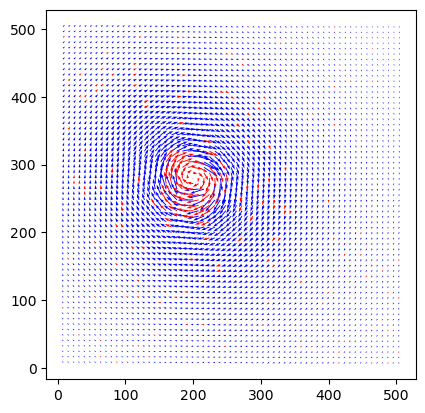
\includegraphics[keepaspectratio]{advanced_files/figure-pdf/cell-2-output-2.png}}

\begin{verbatim}
Image Pair 1
B005_1 B005_2
Saving to results/OpenPIV_results_16_test/field_A0001.txt
\end{verbatim}

\pandocbounded{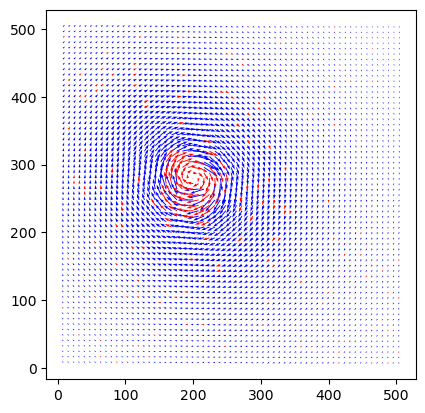
\includegraphics[keepaspectratio]{advanced_files/figure-pdf/cell-2-output-4.png}}

\begin{verbatim}
Image Pair 2
B005_3 B005_4
\end{verbatim}

You can afterwards easily access the computed velocity fields as,

\begin{Shaded}
\begin{Highlighting}[]
\CommentTok{\# Read x, y, u, v variables from the result file}
\NormalTok{data }\OperatorTok{=}\NormalTok{ np.loadtxt(}\StringTok{\textquotesingle{}results/OpenPIV\_results\_16\_test/field\_A0000.txt\textquotesingle{}}\NormalTok{, skiprows}\OperatorTok{=}\DecValTok{1}\NormalTok{)}
\NormalTok{x }\OperatorTok{=}\NormalTok{ data[:, }\DecValTok{0}\NormalTok{]}
\NormalTok{y }\OperatorTok{=}\NormalTok{ data[:, }\DecValTok{1}\NormalTok{]}
\NormalTok{u }\OperatorTok{=}\NormalTok{ data[:, }\DecValTok{2}\NormalTok{]}
\NormalTok{v }\OperatorTok{=}\NormalTok{ data[:, }\DecValTok{3}\NormalTok{]}
\end{Highlighting}
\end{Shaded}

and estimate/show 2d visualizations:

\begin{Shaded}
\begin{Highlighting}[]
\CommentTok{\# Create grid for 2D visualization}
\NormalTok{xi }\OperatorTok{=}\NormalTok{ np.unique(x)}
\NormalTok{yi }\OperatorTok{=}\NormalTok{ np.unique(y)}
\NormalTok{X, Y }\OperatorTok{=}\NormalTok{ np.meshgrid(xi, yi)}
\NormalTok{U }\OperatorTok{=}\NormalTok{ u.reshape(}\BuiltInTok{len}\NormalTok{(yi), }\BuiltInTok{len}\NormalTok{(xi))}
\NormalTok{V }\OperatorTok{=}\NormalTok{ v.reshape(}\BuiltInTok{len}\NormalTok{(yi), }\BuiltInTok{len}\NormalTok{(xi))}
\NormalTok{L2 }\OperatorTok{=}\NormalTok{ np.sqrt(U}\OperatorTok{**}\DecValTok{2} \OperatorTok{+}\NormalTok{ V}\OperatorTok{**}\DecValTok{2}\NormalTok{)}

\NormalTok{fig\_l2, ax\_l2 }\OperatorTok{=}\NormalTok{ plt.subplots(figsize}\OperatorTok{=}\NormalTok{(}\DecValTok{6}\NormalTok{,}\DecValTok{5}\NormalTok{))}
\NormalTok{mesh\_l2 }\OperatorTok{=}\NormalTok{ ax\_l2.pcolormesh(X, Y, L2, shading}\OperatorTok{=}\StringTok{\textquotesingle{}auto\textquotesingle{}}\NormalTok{)}
\NormalTok{plt.colorbar(mesh\_l2, ax}\OperatorTok{=}\NormalTok{ax\_l2, label}\OperatorTok{=}\StringTok{\textquotesingle{}L2 norm\textquotesingle{}}\NormalTok{)}
\NormalTok{ax\_l2.set\_title(}\StringTok{\textquotesingle{}L2 norm of velocity\textquotesingle{}}\NormalTok{)}
\NormalTok{ax\_l2.set\_xlabel(}\StringTok{\textquotesingle{}x\textquotesingle{}}\NormalTok{)}
\NormalTok{ax\_l2.set\_ylabel(}\StringTok{\textquotesingle{}y\textquotesingle{}}\NormalTok{)}
\NormalTok{fig\_l2.tight\_layout()}

\NormalTok{plt.show()  }
\end{Highlighting}
\end{Shaded}

\section{Conclusion}\label{conclusion}

Advanced PIV techniques in OpenPIV provide powerful tools for improving
accuracy and spatial resolution in PIV analysis. Window deformation and
multi-pass processing address limitations of basic PIV analysis, while
comprehensive validation methods ensure reliable vector fields. These
techniques are particularly valuable for complex flows with high shear,
rotation, or spatial gradients.

\section{Assignement}\label{assignement}

Now that your are familiar with the advanced PIV techniques, you will be
asked to analyze some databases of a particular flow: a Lamb-Oseen
vortex flow which is often used for validation due to its well-known
analytical solutions.
\href{https://github.com/jfkrawczynski/um5mee12_jfk/tree/main/images/vortex}{Synthetic
images} are provided for different particle densities, referred as PPP
(Particle Per Pixel).

A \texttt{parameters.mat} is also provided. It provides the particle
individual locations for each time step (30) in the x and y directions.
This file is in a Matlab format but you can access its content as:

\begin{Shaded}
\begin{Highlighting}[]
\ImportTok{import}\NormalTok{ scipy.io}
\NormalTok{mat }\OperatorTok{=}\NormalTok{ scipy.io.loadmat(}\StringTok{\textquotesingle{}parameters.mat\textquotesingle{}}\NormalTok{)}
\end{Highlighting}
\end{Shaded}

Give an evaluation of the velocity vector fields for every test case.
Give some insights about the PIV parameters used for the analyses.
Evaluate the precision of your estimates with regards to the exact
location of the particles as given in \texttt{parameters.mat}.

\part{Practice}

\chapter{Measurements}\label{measurements}

You will conduct experiments with the aim of determining the velocity
field of a flow using PIV. The experiments are carried out in a glass
aquarium measuring 80 x 35 x 40 cm³. An adaptable setup inside the
aquarium allows for generating a recirculating flow. Its modest volume
is well-suited for the space constraints of a practical laboratory
exercise. However, you will notice that it has consequences on the
established flow that you will analyze.

The flow is generated by 4 Aqua Medic Ecodrift 4.3 pumps. These are
propeller pumps commonly used in aquariums. Each pump can produce an
adjustable flow rate of up to approximately 4000 l/h, thus creating a
controlled recirculating flow in the aquarium.

\section{Image recording}\label{image-recording}

The images are acquired by the FlowSense 2M-165 camera, which connects
directly to the computer via a USB 3 port, thus integrating the system
directly within the computer without requiring an additional acquisition
card. This camera offers a resolution of 1920 × 1200 pixels (2.3
megapixels), with a maximum acquisition frequency of 165 frames per
second. It is therefore well-suited for time-resolved PIV for slow to
moderate flows. Its pixel size is 5.9 μm, and the quantum efficiency of
its sensor is greater than 70\%, particularly adapted to the wavelengths
of green light from lasers or LEDs. It uses a CMOS (Complementary
Metal-Oxide-Semiconductor) sensor, which is widely used in modern PIV
systems for its high acquisition rate.

\section{Seeding particles}\label{seeding-particles}

The seeding particles used are polyamide particles (PSP-50, ref.
9080A5011). These particles are produced by polymerization. They are
round, but not perfectly spherical. The size distribution (diameter) of
each particle is between 30 and 70 μm, with an average of 50 μm. Their
density is 1.03 g/cm³, very close to that of water, which therefore
limits their sedimentation. Their refractive index is 1.5.

\section{Light source}\label{light-source}

Illumination is provided by the Fiber-Lite® Mi-LED light generator
(Dolan-Jenner). This system delivers white light with a color
temperature of 5000 K and represents a modern and economical alternative
to conventional 150 W halogen sources.

\section{Assignment}\label{assignment}

During this practical session, you will get familiarized with a simple
experimental setup designed to record particle images of a flow for
which the velocity field is to be estimated.

You will be asked to study three particular flows: 1. a free flow
(without any obstacle) 2. the flow that develops around/behind a
cylinder 3. the flow that develops behind a step

each of which with three flow regimes, i.e.~for three different flow
rates as given by the pumps. Record sufficiently substantial samples to
allow you to subsequently conduct statistical studies.

An in-depth analysis of the obtained images will be expected. Among the
points to be discussed, without being exhaustive, should include: the
average size of the particle images, their density, and the dynamic
range of the gray levels. To do this, you could for example use the
\texttt{regionprops} library adapted from Matlab.

\begin{Shaded}
\begin{Highlighting}[]
\CommentTok{\# Import necessary modules}
\ImportTok{import}\NormalTok{ numpy }\ImportTok{as}\NormalTok{ np}
\ImportTok{import}\NormalTok{ matplotlib.pyplot }\ImportTok{as}\NormalTok{ plt}
\CommentTok{\#matplotlib inline}
\ImportTok{from}\NormalTok{ openpiv }\ImportTok{import}\NormalTok{ tools}
\ImportTok{from}\NormalTok{ skimage.measure }\ImportTok{import}\NormalTok{ label, regionprops}

\CommentTok{\# Load a sample image}
\NormalTok{image }\OperatorTok{=}\NormalTok{ tools.imread(}\StringTok{\textquotesingle{}your image.tif\textquotesingle{}}\NormalTok{)}
\NormalTok{fig, ax }\OperatorTok{=}\NormalTok{ plt.subplots(figsize}\OperatorTok{=}\NormalTok{(}\DecValTok{12}\NormalTok{, }\DecValTok{10}\NormalTok{))}
\NormalTok{ax.imshow(image, cmap}\OperatorTok{=}\NormalTok{plt.cm.gray)}

\CommentTok{\# Use a threshold to segment bright particles}
\NormalTok{threshold }\OperatorTok{=}\NormalTok{ np.percentile(image, }\DecValTok{90}\NormalTok{)  }\CommentTok{\# adjust percentile as needed}
\NormalTok{binary\_img }\OperatorTok{=}\NormalTok{ image }\OperatorTok{\textgreater{}}\NormalTok{ threshold}

\NormalTok{label\_img }\OperatorTok{=}\NormalTok{ label(binary\_img, background}\OperatorTok{=}\DecValTok{0}\NormalTok{) }\CommentTok{\# adjust background as needed}
\NormalTok{regions }\OperatorTok{=}\NormalTok{ regionprops(label\_img, intensity\_image}\OperatorTok{=}\NormalTok{image)}

\ControlFlowTok{for}\NormalTok{ props }\KeywordTok{in}\NormalTok{ regions:}
    \CommentTok{\# Use weighted centroid for better accuracy}
\NormalTok{    y0, x0 }\OperatorTok{=}\NormalTok{ props.weighted\_centroid}
\NormalTok{    ax.plot(x0, y0, marker}\OperatorTok{=}\StringTok{\textquotesingle{}x\textquotesingle{}}\NormalTok{, color}\OperatorTok{=}\StringTok{\textquotesingle{}r\textquotesingle{}}\NormalTok{, markersize}\OperatorTok{=}\DecValTok{6}\NormalTok{)}

\NormalTok{plt.show()}
\end{Highlighting}
\end{Shaded}

You will then work on the collected databases by implementing a method
for evaluating velocity fields using OpenPIV. You will detail the method
used, emphasizing the choice of parameters for the PIV analysis.

Finally, you will develop an analysis of the obtained velocity fields
based on, among other things, considerations discussed in class with
Mr.~Druault.

\bookmarksetup{startatroot}

\chapter*{References}\label{references}
\addcontentsline{toc}{chapter}{References}

\markboth{References}{References}

\phantomsection\label{refs}
\begin{CSLReferences}{1}{0}
\bibitem[\citeproctext]{ref-adrian1991particleimaging}
Adrian, R. J. 1991. {``Particle-Imaging Techniques for Experimental
Fluid Mechanics.''} \emph{Annual Review of Fluid Mechanics} 23 (1):
261--304. \url{https://doi.org/10.1146/annurev.fl.23.010191.000245}.

\bibitem[\citeproctext]{ref-huang1997errors}
Huang, Dabiri, H. 1997. {``On Errors of Digital Particle Image
Velocimetry.''} \emph{Measurement Science and Technology} 8 (12):
1427--39. \url{https://doi.org/10.1088/0957-0233/8/12/1427}.

\bibitem[\citeproctext]{ref-raffelParticleImageVelocimetry2007}
Raffel, Willert, M. 2007. \emph{Particle Image Velocimetry: A Practical
Guide}. springer.

\bibitem[\citeproctext]{ref-rougierTenSimpleRules2014}
Rougier, Michael Droettboom, Nicolas P. 2014. {``Ten Simple Rules for
Better Figures.''} \emph{PLOS Computational Biology} 10 (9).
\url{https://doi.org/10.1371/journal.pcbi.1003833}.

\bibitem[\citeproctext]{ref-rougierScientificVisualizationPython2021}
Rougier, Nicolas P. 2021. \emph{Scientific Visualization: Python +
Matplotlib}. CRC Press.

\end{CSLReferences}




\end{document}
